\chapter{Simulation du SDHCAL}
\label{chap.simulation}
La simulation est un aspect très important dans les expériences de physique des particules. En effet, la conception et l'optimisation d'un détecteur s'appuient toujours sur la simulation qui va permettre une estimation rapide des performances, des coûts de l'expérience. Les simulations sont aussi massivement utilisées dans l'analyse des données pour améliorer les algorithmes d'analyses, pour confirmer ou non la présences de nouvelle physique, pour estimer les biais... C'est pourquoi avoir une simulation la plus réaliste possible est un enjeu très importants. Dans ce chapitre, nous présenterons les modèles utilisés pour la simulation des gerbes hadroniques. Puis nous détaillerons la simulation du prototype SDHCAL et nous expliquerons les différentes étapes de la modélisation de la réponse des GRPC aux particules chargées. Enfin quelques des comparaisons entre les données et la simulation seront présentées. 
\minitoc
\newpage

%%%%%%%%%%%%%%%%%%%%%%%%%%%%%%%%%%%%%%%%%%%%%%%

\section{Les modèles de simulation des gerbes hadroniques}
La collaboration GEANT4 \cite{geant4} fournit un logiciel rassemblant de nombreux modèle théoriques et phénoménologiques qui décrivent les interactions de particules avec la matière. Ces modèles n'étant valable que sur certaines gammes d'énergies (cf. figure~\ref{fig.model}), l'utilisateur doit les combiner pour simuler un phénomène physique. La collaboration GEANT4 fournit aussi un certain nombre de listes physiques utilisant et définissant des transitions entre ces modèles (cf. section~\ref{sec.listphys}).
\begin{figure}[!ht]
  \begin{center}
    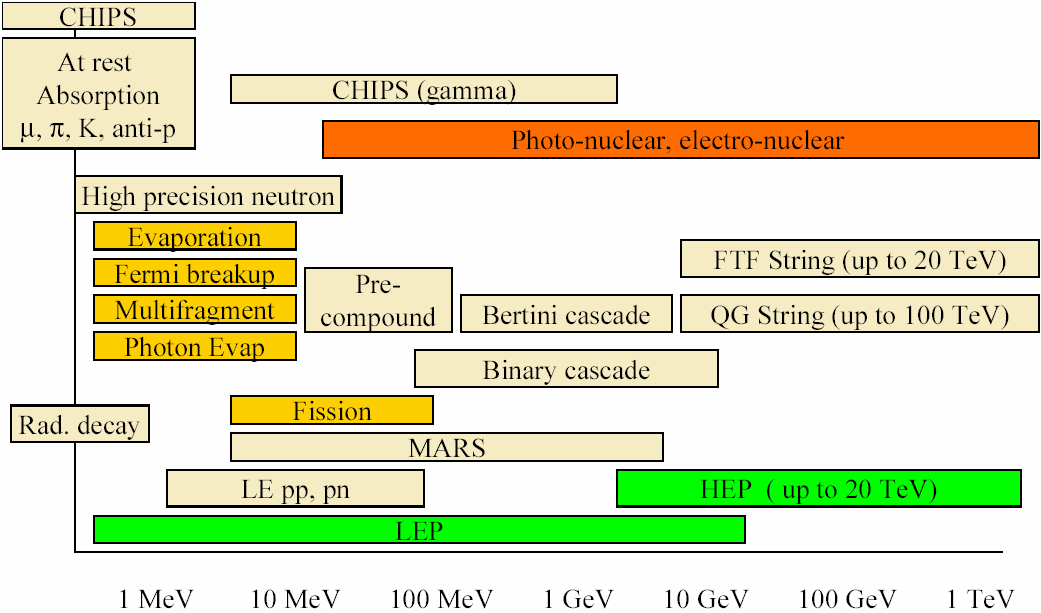
\includegraphics[width=.8\textwidth]{Digitizer/figs/HadronicModelsInventory.jpg}
    \caption{Les modèles utilisés dans GEANT4.}
    \label{fig.model}
  \end{center}
\end{figure}
\\
Les principaux modèles pour les interactions hadroniques de haute énergie avec la matière sont les modèle de cordes partoniques (cf. section~\ref{sec.parton}) qui sont valables pour des énergies supérieur à $5-10$ GeV. Les interactions aux énergies intermédiaires (100 MeV < E < 10 GeV) sont simulées avec les modèle de cascade intranucléaires (cf. section~\ref{sec.inucl}). Pour traiter les noyaux excités par des collisions de plus haute énergie et les interactions en dessous de 200 MeV, une famille de modèle de désexcitation nucléaire (fission, évaporation nucléaire\dots) est disponible. Les interactions des neutrons de basses énergies (E<20 MeV) peuvent être simulées avec des modèles de haute précision pour neutrons où un grand nombre de sections efficaces ont été tabulés. L'utilisation ou non de ces modèles de haute précision pour les neutrons aura des conséquences sur le temps de calcul, sur la réponse simulée du détecteur ou sur la topologie des gerbes\dots
\subsection{Modèles de cordes partoniques}
\label{sec.parton}
Les modèles de cordes partoniques permettent de simuler les réaction de hautes énergies de hadrons avec des noyaux. Les deux principaux modèles utilisés dans GEANT4 sont les modèles QGS (Quark Gluon String) et FTF (Fritiof) \cite{geant4_parton}. Le résultat de l'interaction d'un hadron avec un noyau est une ou plusieurs cordes excitées. Une corde est un segment où chacune des deux extrémités est un quark ou un di-quark se déplaçant dans des directions opposées. Les noyaux sont modélisés comme un ensemble de nucléons dont les positions sont aléatoirement choisies en utilisant une distribution de densité. Pour les noyaux lourd (A>16), une distribution de densité de la forme du potentiel de Wood-Saxon est utilisée : 
\begin{equation}
  \rho(r_i)=\frac{\rho_0}{1+exp[(r_i-R)]/a}
\end{equation}
où $R$ et $a$ dépendent de la masse du noyau. Pour les noyau léger une distribution de densité venant du modèle d'oscillateur harmonique est utilisée : 
\begin{equation}
  \rho(r_i)=(\pi R'^2)^{-3/2}exp(-r_i^2/R'^2)
\end{equation}
avec $R'$  qui dépend de la masse du noyau.
Pour calculer le paramètre d'impact avec les nucléons, ces deux distribution de densité sont réduites dans un plan perpendiculaire à la direction de la particule incidente. La probabilité de collision entre entre le hadron et un nucléon est calculée en utilisant une distribution gaussienne pour les fonctions d'onde du hadron et des nucléons. Ces probabilités sont utilisée pour connaître le nombre de nucléons participant à la réaction dans le noyau.\\
Des cordes sont ensuite crées, les quarks du hadron incident sont aléatoirement répartis entre celles-ci. Un modèle de fragmentation longitudinal de cordes est ensuite utilisé où ces cordes sont séparées en hadrons et en une nouvelle corde. Une corde se fragmente en une paire quark-antiquark $q-\bar q$ ou diquark-antidiquark $qq-\bar q \bar q$ \cite{geant4_reference}. Les probabilités relatives de création des quark ou diquark sont :
\begin{equation}
  u:d:s:qq = 1:1:0.35:0.1
\end{equation}
La paire de quark-antiquark (ou diquark-antidiquark) créée est placée entre la précédente paire. Une moitié de ces nouvelles paires sont utilisées pour créer un hadron tandis que les autres constituants créent une nouvelle corde. Ce processus se répète jusqu'à ce que l'énergie d'une corde ne soit pas suffisante pour créer un hadron.\\
Après l'interaction du noyau avec la particule incidente, celui-ci sera dans un état excité. Le retour à l'état fondamental du noyau est simulée avec des modèle de fragmentation et de désexcitation nucléaire.
\begin{table}[!ht]
  \begin{center}
    \begin{tabular}{c|c|c}
      Particule & QGS & FTF\\
      \hline
      $k+$ & $12\ GeV\ -\ 100\ TeV$ & $4\ GeV\ -\ 100\ TeV$\\
      $k-$ & $12\ GeV\ -\ 100\ TeV$ & $4\ GeV\ -\ 100\ TeV$\\
      $\lambda$ & $ $ & $2\ GeV\ -\ 100\ TeV$\\
      $\pi+$ & $12\ GeV\ -\ 100\ TeV$ & $4\ GeV\ -\ 100\ TeV$\\
      $\pi-$ & $12\ GeV\ -\ 100\ TeV$ & $4\ GeV\ -\ 100\ TeV$\\
      $neutron$ & $12\ GeV\ -\ 100\ TeV$ & $4\ GeV\ -\ 100\ TeV$\\
      $proton$ & $12\ GeV\ -\ 100\ TeV$ & $4\ GeV\ -\ 100\ TeV$\\
      $ion$ & $ $ & $2\ GeV\ -\ 100\ TeV$\\
    \end{tabular}
  \end{center}
  \caption{Chambers list where threshold are changed.}
  \label{tab.partonModelTable}
\end{table}
\subsection{Le modèles de cascade intranucléaire de Bertini}
\label{sec.inucl}
Il a été montré dans \cite{bertini} en 1969 qu'un modèle de cascade intranucléaire décrivait relativement bien les interactions de nucléons de 100 MeV à 2 GeV avec des noyaux. Ces réactions sont caractérisées par une rapide ($10^{-23}-10^{-22} s$) cascade intranucléaire laissant les noyaux dans un état excité, suivi d'une phase plus lente ($10^{-18}-10^{-16} s$) d'évaporation nucléaire. blabblba geant4 deux modèle...
\begin{figure}[!ht]
  \begin{center}
    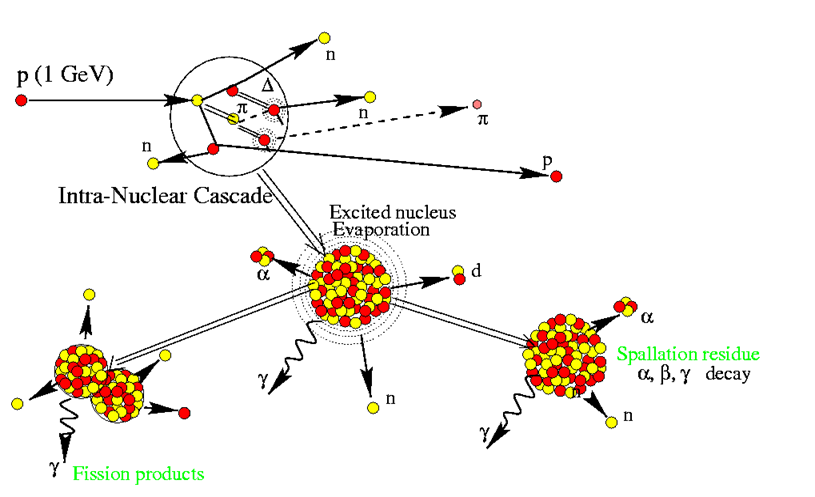
\includegraphics[width=.8\textwidth]{Digitizer/figs/intraNucl.png}
    \caption{Schéma d'explication du modèle de Bertini. Un hadron de 400 MeV crée une cascade intraucléaire.}
    \label{fig.g4bertini}
  \end{center}
\end{figure}
\subsubsection{Bertini}
Ce modèle a depuis été étendu et est valable pour des particules incidentes ($p,n,\pi,K,\Delta,\Sigma,\Xi,\Omega$ et $\gamma$) avec une énergie cinétique comprise entre 100 MeV et 10 GeV~\cite{geant4_bertini}. Ce modèle est applicable lorsque la longueur d'onde de de Broglie de la particule incidente est de l'ordre de la distance moyenne entre les nucléons du noyau. Le noyau cible est modélisé par jusqu'à six couche concentrique de densité constante. La cascade commence lorsque une particule incidente rencontre un nucléon du noyau cible et produit des particules secondaires. Ces particules secondaires interagissent alors avec les autres nucléons, sont absorbés ou s'échappent du noyau. La cascade prend fin lorsque toutes les particules secondaires sont soit absorbées soit se sont échappées. La figure~\ref{fig.g4bertini} illustre le phénomène de cascade intranucléaire.
\subsubsection{Binary}
Dans GEANT4, un autre modèle de cascade intranucléaire est disponible et est utilisé par certaine liste physique. C'est le modèle de cascade binaire. 
\subsection{Les listes physiques}
\label{sec.listphys}
\begin{figure}[!ht]
  \begin{center}
    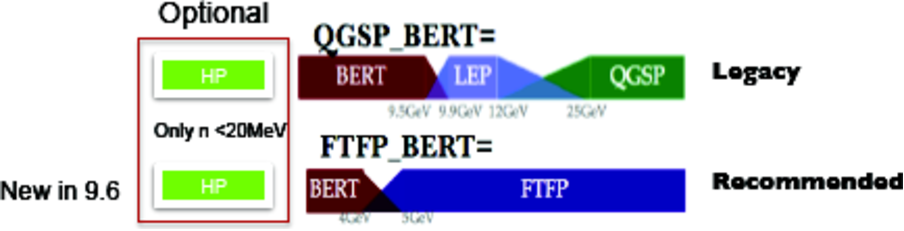
\includegraphics[width=.8\textwidth]{Digitizer/figs/physics_list_G4.pdf}
    \caption{Liste physique.}
    \label{fig.g4list}
  \end{center}
\end{figure}

%%%%%%%%%%%%%%%%%%%%%%%%%%%%%%%%%%%%%%%%%%%%%%%

\section{La simulation du prototype}
La simulation du prototype SDHCAL a été réalisé avec un programme basé sur GEANT4 \cite{geant4}. La géométrie du détecteur est décrite dans ce programme avec de nombreux détails. Les compositions chimiques, les densités des matériaux du prototypes sont utilisés. Ces informations seront utilisées par GEANT4 pour des calculs de sections efficaces lors de la propagation des particules dans le détecteur. Le champ électrique entre les deux électrodes de verre des GRPC n'est pas simulé. Les avalanches issues des ionisations du gaz par les particules incidentes sont modélisés par un algorithme dédié qui sera décrit dans la partie~\ref{sec.digit-algo} de ce chapitre. La trajectoire des particules primaires et secondaires est segmentée dans GEANT4. A chaque interaction avec les matériaux du détecteur un nouveau segment est créé. La création d'un nouveau segment se fait aussi à chaque fois qu'une particule change de volume (e.g. passant du verre au gaz). La liste des segments se trouvant dans le milieu actif du détecteur (le gaz entre les électrodes pour le SDHCAL) est alors enregistrée. Les informations stockées pour ces segments sont les suivantes: les coordonnées des positions du début et de la fin du segment; l'énergie perdue par la particule le long du segment; la nature de la particule; le temps d’occurrence du segment relatif au moment où la particule primaire a été générée. 
Cette liste de segment est ensuite utilisée comme point de départ de l’algorithme qui modélise la réponse des GRPC au particules chargées.

%%%%%%%%%%%%%%%%%%%%%%%%%%%%%%%%%%%%%%%%%%%%%%%

\section{Modèlisation de la réponse des GRPC au particules chargées}
Nous venons de voir que le résultat du programme de simulation du SDHCAL est une liste de segments correspondant à une partie de la trajectoire d'une particule dans le détecteur. Nous avons vu que l'énergie déposée par ces segments étaient disponible alors que dans le cas du SDHCAL la charge induite sur les carreaux de cuivre est mesurée. De plus, le phénomène de multiplicité introduit au chapitre~\ref{chap.sdhcal} n'est pas pris en compte par GEANT4. 
\label{sec.digit-algo}
%%%%%%%%%%%%%%%%%%%%%%%%%%%%%%%%%%%%%

\subsection{Algorithme SimDigital}
\label{sec.algo}
La modélisation est faite à l'aide d'un algorithme appelé SimDigital qui est un processeur Marlin \cite{marlin} disponible dans le paquet MarlinReco \cite{marlinreco} de l'ILCSoft \cite{ilcsoft}. Le but de cet algorithme est de simuler la réponse des GRPC lors du passage de particules chargées dans la l'intervalle de gaz. Les différentes étapes de l’algorithme sont les suivantes:
\begin{enumerate}[~~1-]
\item La fenêtre en temps utilisée dans la procédure de reconstruction des événements décrites dans la partie~\ref{sec.trivent} du chapitre~\ref{chap.sdhcal} est de 1000 $ns$. Ainsi, les particules interagissant tardivement dans le détecteur comme les neutrons peuvent ne pas être associées à l’événement. Pour prendre cet effet en compte, les segments avec un temps d’occurrence supérieur à 1000 $ns$ sont supprimés.
\item \label{it.start} Un canal de lecture $C_0$ où un ou plusieurs segments ont traversé le gaz est sélectionné. La longueur de ses segments est alors calculée.
\item La longueur de certains des segments dans le gaz peut être très petite. Ce phénomène peut arriver aléatoirement lors de la propagation des particules par GEANT4. Cependant la majorité des cas où ce phénomène s'observe, s'explique par le changement de volume d'une particule. La figure~\ref{fig.map_and_length_vs_deltaz}(a) présente la longueur des segments en fonction de la distance ($\Delta_z$) entre la position du milieu du segment et le milieu de la couche de gaz. Cette figure montre qu'une grande fraction des segments de faible longueur sont proches des deux électrodes en verre ($|\Delta_z|\simeq0.6~mm$). Ces segments de longueur presque nulle n'ont pas de raison de déclencher une avalanche dans le gaz. Les segments de longueur est inférieure à une longueur donnée $l_{min}$ sont donc supprimés.
  \begin{figure}[!ht]
    \subfigure[]{\includegraphics[width=0.5\textwidth]{Digitizer/figs/sstepLength_vs_deltaZ_ZOOM.pdf}}
    \subfigure[]{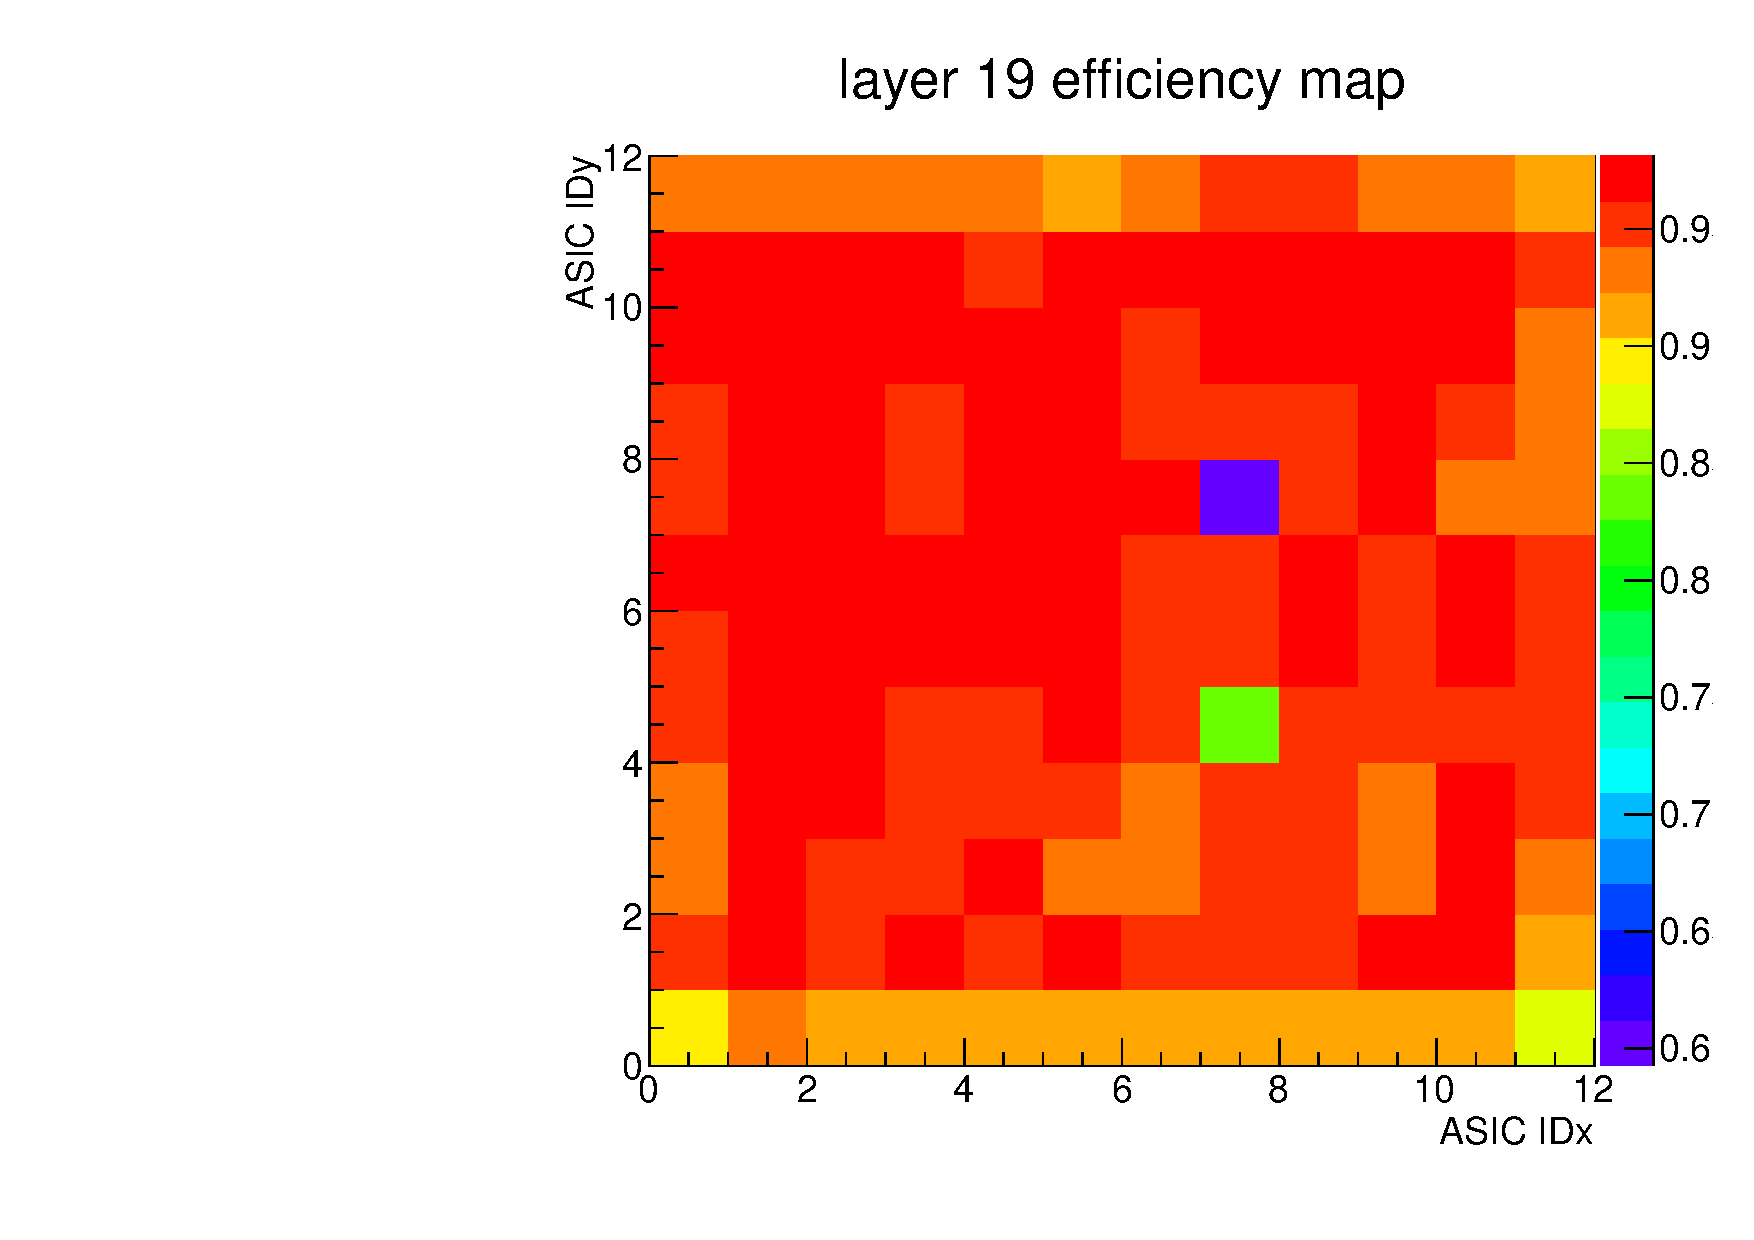
\includegraphics[width=0.5\textwidth]{Digitizer/figs/layer19map.pdf}}
    \caption{(a): Longueur des segments en $mm$ en fonction de $\Delta_z$ en $mm$. Cette figure est centrée sur la région des segments de faible longueur pour mettre en évidence le fait que la plupart des segments de longueur nulle (ou presque) sont localisé sur les bords de la couche de gaz ($|\Delta_z|\simeq0.6\ mm$). (b): Exemple d'une carte d'efficacité des ASICs.}
    \label{fig.map_and_length_vs_deltaz}
  \end{figure}
\item Les cartes d'efficacité des ASIC du prototype déterminées grâce à l'étude des muons décrite dans la partie~\ref{sec.muons} du chapitre~\ref{chap.sdhcal}, sont utilisées pour prendre en compte les effets des $quenchers$ ($CO_2$,$SF_6$). En effet, les propriétés de ces deux gaz (capture des photons et d'électrons) ne sont pas incluses dans GEANT4. De plus, l'utilisation de ces cartes d’efficacité permet d'éviter la présence de signal dans les canaux électroniques hors d'usage ou masqués. Ainsi, lorsqu'un segment est dans une région du détecteur où l'efficacité est de 50\% alors ce segment a 50\% de chance d'être conservé. La figure~\ref{fig.map_and_length_vs_deltaz} montre un exemple de carte d'efficacité d'une chambre du prototype SDHCAL.
\item La charge induite pour chaque segment est alors aléatoirement choisis dans une distribution de Polya: 
  \begin{equation}
    \label{eq.polya}
    P(q)=[\frac{q}{\bar q}(1+\theta)]^{\theta}e^{[-\frac{q}{\bar q}(1+\theta)]}
  \end{equation}
  où $\bar q$ est la valeur moyenne et $\theta$ un paramètre libre lié à la largeur de la distribution. Cette charge induite est ensuite corrigée: 
  \begin{equation}
    \label{eq.lengthcorrection}
    Q_{corr} = \left\{ \begin{array}{rl}
      Q_{ind}(\frac{d_s}{d_{gap}})^\kappa &\mbox{ si $\frac{d_s}{d_{gap}}>1$} \\
      Q_{ind} &\mbox{ sinon}
    \end{array} \right.
  \end{equation}
  où $d_s$ correspond à la longueur du segment, $d_{gap}$ à l'épaisseur de la couche de gaz (1.2 $mm$) et $\kappa$ un paramètre libre. L'effet et l'importance de cette correction seront discuté dans la partie~\ref{sec.param} de ce chapitre.
\item Dans les gerbes hadroniques et électromagnétiques, les particules chargés peuvent être très proches. Ainsi les avalanche induites dans le gaz par ces particules peuvent se chevaucher. Cependant, dans le régime avalanche le signal induit par ces particules n'est pas équivalent à la somme des signaux induits par ces particules pris individuellement. Pour simuler cet effet, lorsque la distance entre deux segments est inférieure à une valeur $d_{cut}$, le segment dont la charge induite ($Q_{corr}$) est la plus faible, est supprimé. Ce filtre permet aussi de supprimer un ou plusieurs segments provenant d'une seule particule. En effet, une interaction entre une particule chargée et le gaz peut avoir lieu dans GEANT4. Ainsi plusieurs segments seraient créés et pourraient déclencher plusieurs avalanches alors qu'une seule particule est passée.
\item \label{it.spliting} La charge induite est ensuite réparti sur le canal de lecture $C_0$  et sur les canaux voisins. Les canaux voisins correspondent au cellules dans le même plan que $C_0$ à une distance inférieur à une valeur $r_{max}$. Le rapport suivant est alors calculé pour chaque canal:
  \begin{equation}
    \label{eq.ratio}
    R_i = \frac{\int_{a_i}^{b_i}\int_{c_i}^{d_i}\sum_{j=0}^{n}\alpha_j e^{ \frac{(x_0-x)^2+(y_0-y)^2}{\sigma_j^2}}dxdy}{N}
  \end{equation}
  où $a_i,\ b_i,\ c_i,\ d_i$ sont les positions des bords de la cellule $i$, $(x_0,y_0)$ sont les coordonnées du milieu du segment et N un facteur de normalisation définit comme: 
  \begin{equation}
    \label{eq.norm}
    N=\int_{-r_{max}}^{+r_{max}}\int_{-r_{max}}^{+r_{max}}\sum_{j=0}^{n}\alpha_j e^{ \frac{(x_0-x)^2+(y_0-y)^2}{\sigma_j^2}}dxdy
  \end{equation}
\item Pour chaque canal ($C_0$ et ses voisins), sa charge induite est augmenté d'une valeur $R_iQ_{corr}$.
\item L'opération est répétée à partir de l'étape~\ref{it.start} pour tous les canaux avec des segments.
\item Les seuils sont finalement appliqués pour tous les canaux. Les canaux pour lesquels la charge induite est inférieur à la valeur du premier seuil sont supprimés. Les canaux restant sont alors étiquetés selon la valeur de leur charge induite. 
\end{enumerate}

%%%%%%%%%%%%%%%%%%%%%%%%%%%%%%%%%%%%%

\subsection{Paramétrisation de l'algorithme}
\label{sec.param}
Nous avons vu les différentes étapes de l'algorithme responsable de la simulation de la réponse des GRPC au passage de particules chargées. Cet algorithme introduit de nombreux paramètres. Les méthodes utilisés pour obtenir la meilleur paramétrisation sont décrites dans la section suivantes. 
%%%%%%%%%%%%%%%%%%%%%%%%%%%%%%%%%%%%%

\subsubsection{Mesure du spectre de charge}
% 
\label{sec.polya}
Le régime utilisé pour les GRPCs du prototype est le régime avalanche saturée. Ce régime à été décrit dans \cite{abbresciaPolya} et il a été montré qu'une distribution de Polya (cf. Eq.~\ref{eq.polya}) s'ajuste bien aux spectres de charge expérimentales. Il n'était pas possible de faire une mesure directe du spectre de charge avec une chambre du prototype. Cette mesure qui nécessite une lecture analogique d'une GRPC avait été réalisé avec une chambre différentes de celles du prototype. La chambre utilisé était plus petite, le signal était enregistré avec un seul canal de lecture de $8 \times 8 ~cm^{2}$. Le mélange de gaz et la haute tension appliquée était différents. Nous étions donc contraints de refaire la mesure du spectre de charge pour les GRPCs du prototype avec une autre méthode. La méthode que nous avons utilisé est un scan en seuil. Cette méthode consiste à étudier l'efficacité de détection de muons en fonctions de la valeur des seuils. Nous avons choisis 9 chambres dans lesquels nous avons fait varier la valeur du seuil 1, 2 ou 3. Le tableau~\ref{tab.thrScan} montre quel seuil nous avons fait varier dans quelle chambre.
\begin{table}[!ht]
  \begin{center}
    \begin{tabular}{c|c}
      Seuil & Numéro de chambre\\
      \hline
      $1$ & $6,~16,~30$\\
      $2$ & $10,~22,~34$\\
      $3$ & $14,~26,~38$\\
    \end{tabular}
  \end{center}
  \caption{Liste des chambres utilisées pour le scan en seuil.}
  \label{tab.thrScan}
\end{table}
Pour étudier l'efficacité de détection de ces chambres, nous avons utilisé les autres pour reconstruire les traces des muons. La première étape de la reconstruction des traces est de regrouper les coups lorsqu'ils sont dans le même plan et lorsqu'ils se touchent. 
%un schéma de clusters...
Le barycentre de ces groupes de coups est alors utilisé pour effectuer une régression linéaire et ainsi calculer la position attendue du point d'impact de la trace dans les plans étudiés. Une chambre est alors comptée comme efficace si un groupe de coups est trouvé dans un rayon de $2.5~cm$ autour de la position attendue. La figure~\ref{fig.thrScan}(a) montre les efficacités moyennes en fonction du seuil. 
Cette courbe est ensuite ajustée avec le fonction suivante:
\begin{equation}
  \label{eq.fitScan}
  \varepsilon(q)=\varepsilon _0 - c\int_0^q{[\frac{q'}{\bar q}(1+\theta)]^{\theta}e^{[-\frac{q'}{\bar q}(1+\theta)]}dq'}
\end{equation}
où $\bar q$ et $\theta$ sont les paramètre de la distribution de Polya, $c$ est un paramètre libre et $\varepsilon_0$ la valeur asymptotique de l'efficacité.
\begin{figure}[!ht]
  \subfigure[]{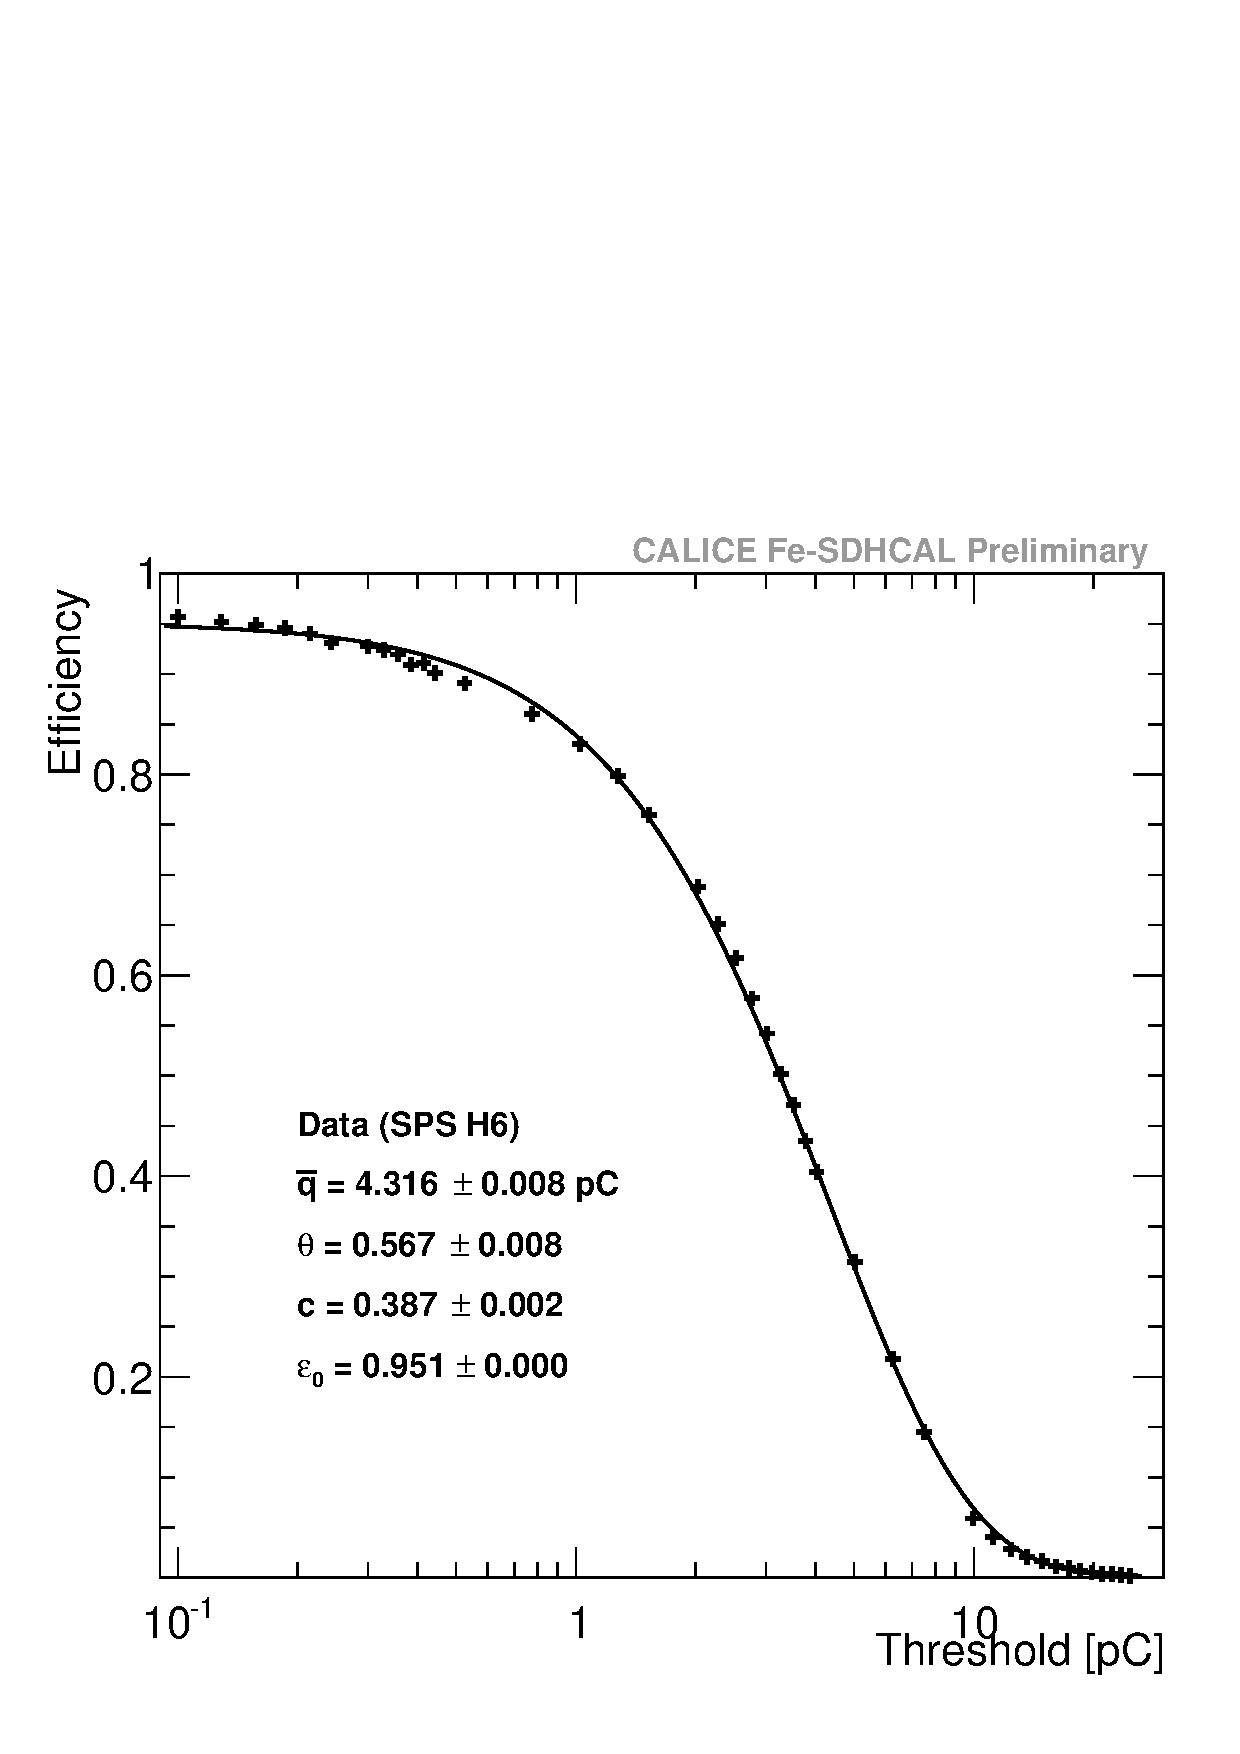
\includegraphics[width=.5\textwidth]{Digitizer/figs/thrScanDat.pdf}}
  \subfigure[]{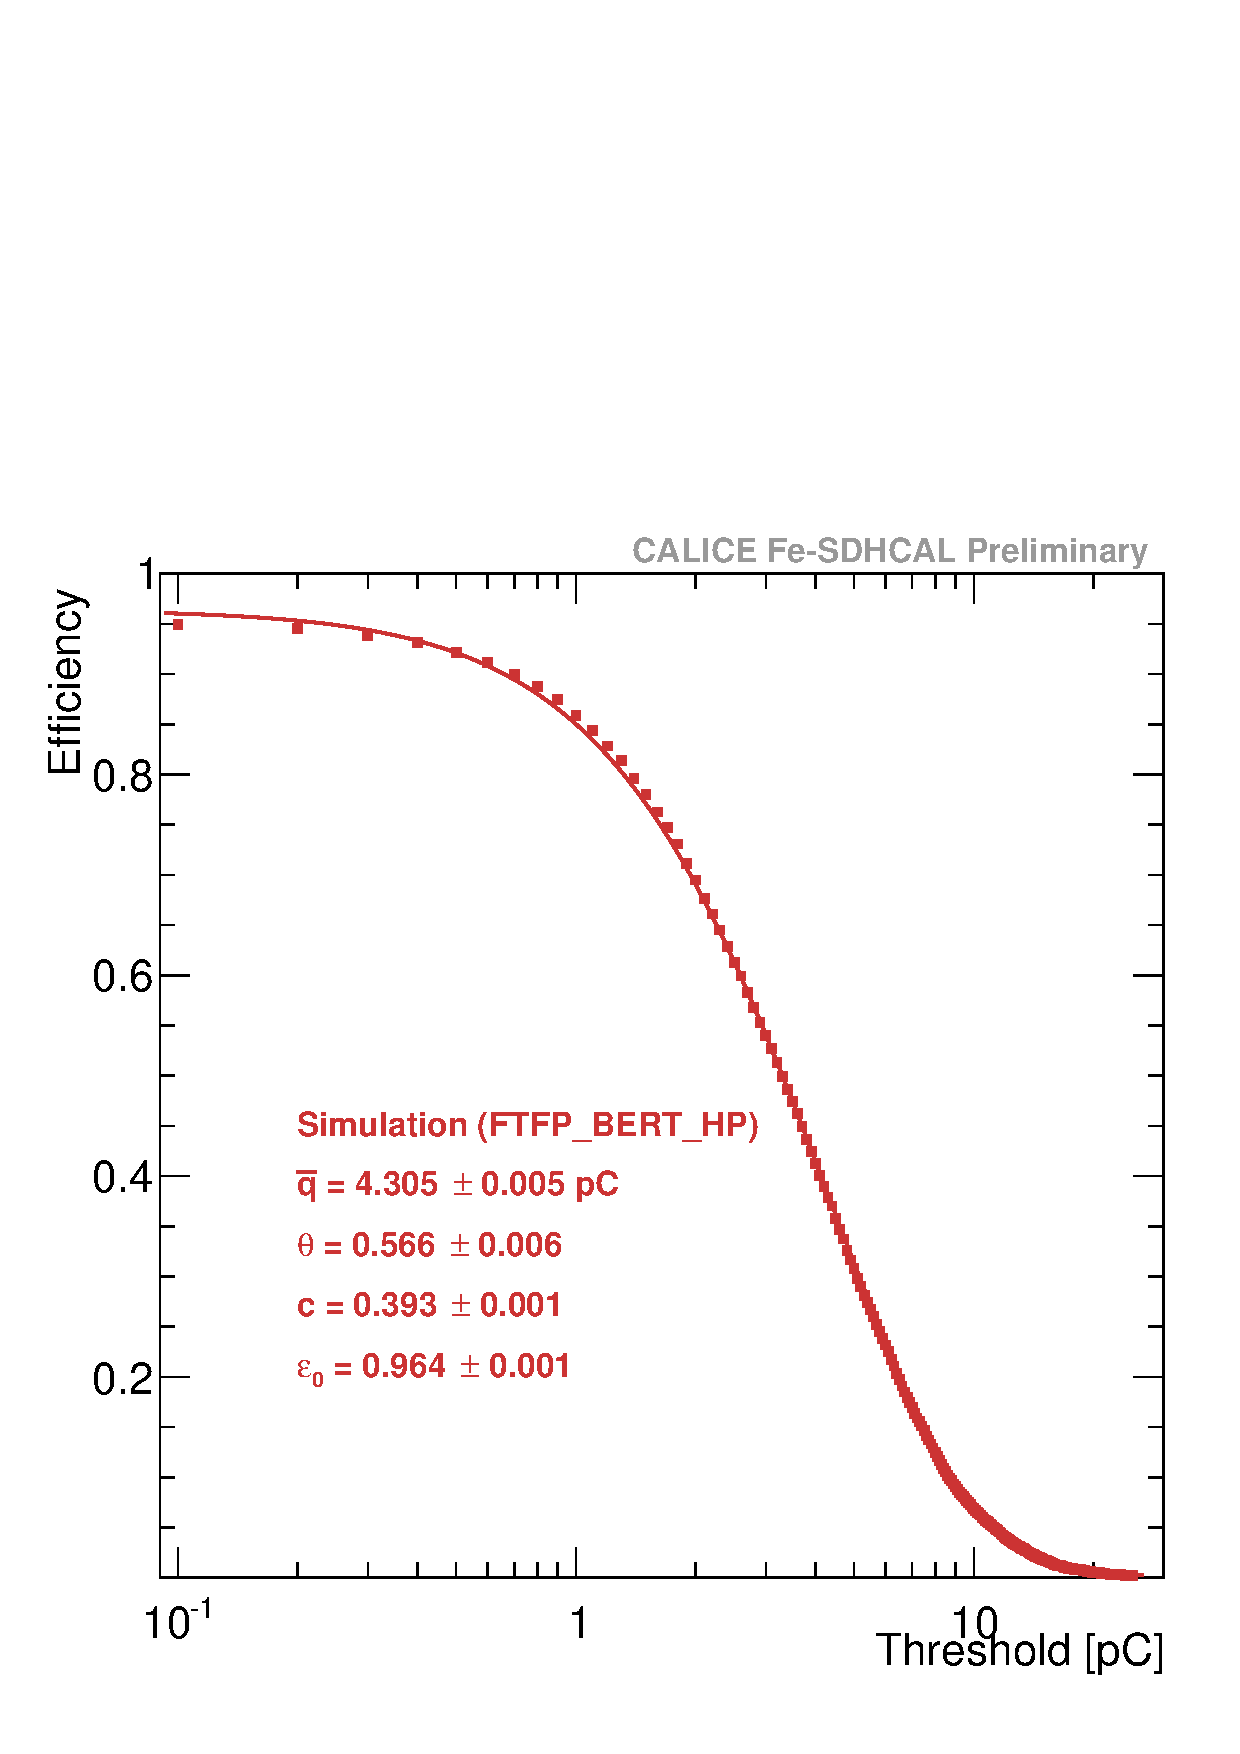
\includegraphics[width=.5\textwidth]{Digitizer/figs/thrScanSim.pdf}}
  \caption{(a) Résultats du scan en seuil pour les données (a) et pour la simulation (b). \label{fig.thrScan}}
\end{figure}
 La même procédure est réalisé avec la simulation. Les paramètre $\bar q$ et $\theta$ sont réglés pour reproduire les résultats obtenus avec les données du prototype. La figure~\ref{tab.thrScan}(b) montre la courbe d'efficacité moyenne en fonction du seuil pour la simulation. Le tableau~\ref{tab.inputPolya} présente le valeur d'entrée des paramètres de la distribution de Polya utilisée dans l'algorithme.
\begin{table}[!ht]
  \begin{center}
    \begin{tabular}{c|c}
      Paramètre & Valeur\\
      \hline
      $\bar q$ & $1.05$\\
      $\theta$ & $4.53 pC$\\
    \end{tabular}
  \end{center}
  \caption{Valeur d'entrée des paramètres de la Polya utilisé par l'algorithme SimDigital.}
  \label{tab.inputPolya}
\end{table}
 Cependant, les valeurs des paramètres obtenues avec l'ajustement (cf. Eq.~\ref{eq.fitScan}) sont sensiblement différentes des valeurs d'entrées. Ceci vient de l'étalement de la charge induite sur plusieurs canaux de lecture (cf. étape~\ref{it.spliting} de la section~\ref{sec.algo} de ce chapitre). Ainsi une fraction de la charge induite est perdue lorsque les seuils sont appliqués.
%%%%%%%%%%%%%%%%%%%%%%%%%%%%%%%%%%%%%

\subsubsection{Répartition de la charge}
Les paramètres introduits dans les équations~\ref{eq.ratio} et~\ref{eq.norm} sont réglés pour reproduire la multiplicité moyenne et le nombre de coups dans les gerbes électromagnétiques. La multiplicité est définie comme le nombre coups dans les groupes définis précédemment, lorsqu'une seule particule traverse la couche de gaz. La multiplicité moyenne pour chaque GRPC est calculée en utilisant la même méthode de reconstruction de trace décrit dans la section~\ref{sec.polya}. De nombreuses configurations de ces paramètres ont été testées pour reproduire à la fois la multiplicité moyenne et le nombres de coups dans les gerbes électromagnétiques. Le paramètre $n$ de l'équation~\ref{eq.ratio} est fixé à 2. Il n'était pas possible de reproduire les différentes observables des données avec $n=1$. Une augmentation de la valeur de ce paramètre n'apporte pas d'amélioration et ajoute des difficultés pour paramétrer l'algorithme. Le tableau~\ref{tab.splitting} présentes les valeurs d'entrées des paramètres $\alpha$ et $\sigma$.
\begin{table}[!ht]
  \begin{center}
    \begin{tabular}{c|c}
      Paramètre & Valeur\\
      \hline
      $\alpha_0$ & $1.0$\\
      $\sigma_0$ & $1.0~mm$\\
      $\alpha_1$ & $0.00083$\\
      $\sigma_1$ & $9.7~mm$\\
    \end{tabular}
  \end{center}
  \caption{Valeur d'entrée des paramètres introduit dans l'équation~\ref{eq.ratio}.}
  \label{tab.splitting}
\end{table}
Le paramètre $r_{max}$ est fixé à 30 $mm$. Une augmentation de cette valeur n’entraîne pas de variation significative sur le résultat final de la simulation. En effet, la quantité de charge déposée sur les carreaux éloignés de plus de 30 $mm$ de la particule est négligeable (avec la paramétrisation actuelle). La figure~\ref{fig.eff_mul_layer} montre l'efficacité (fig.~\ref{fig.eff_mul_layer}(a)) et la multiplicité (fig.~\ref{fig.eff_mul_layer}(b)) moyenne par chambre pour les données et la simulation.
\begin{figure}[!ht]
  \subfigure[]{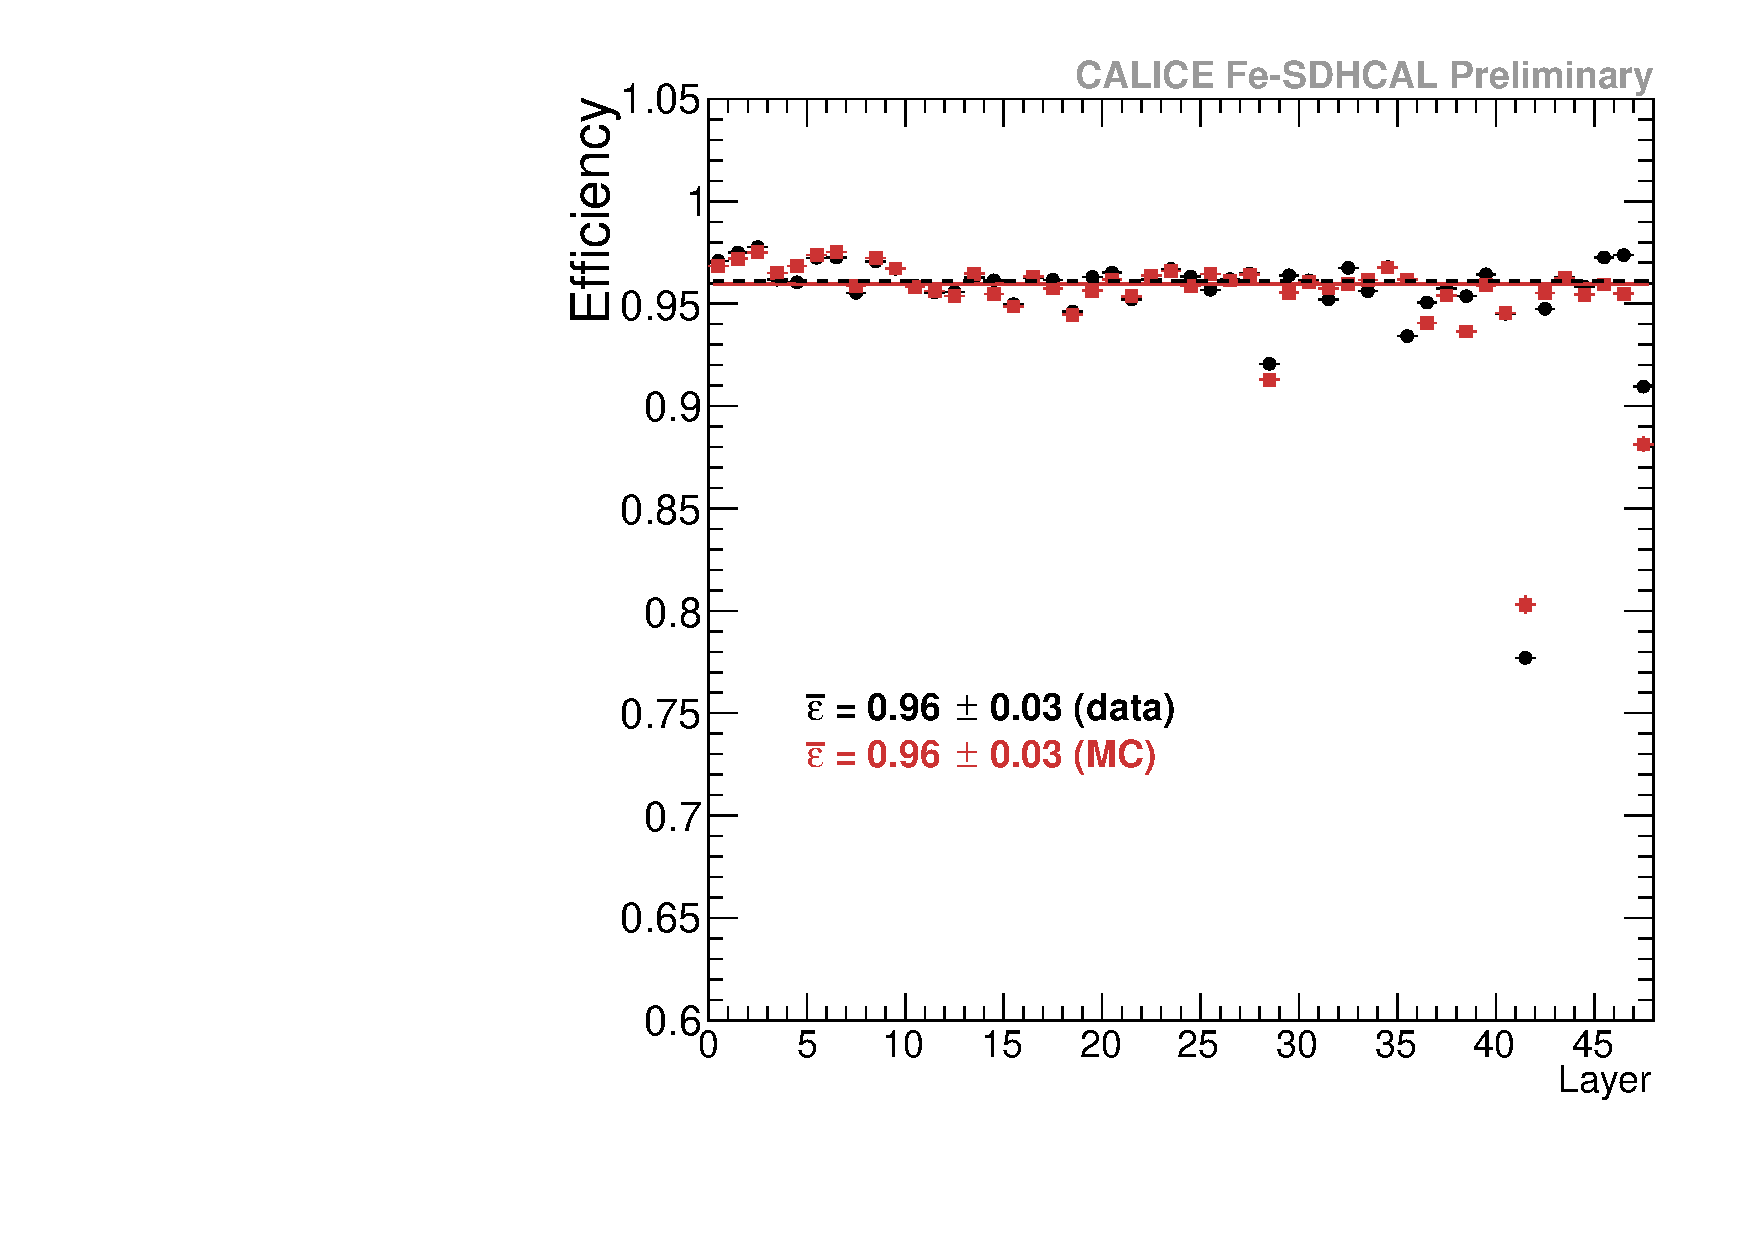
\includegraphics[width=.5\textwidth]{Digitizer/figs/effLayer.pdf}}
  \subfigure[]{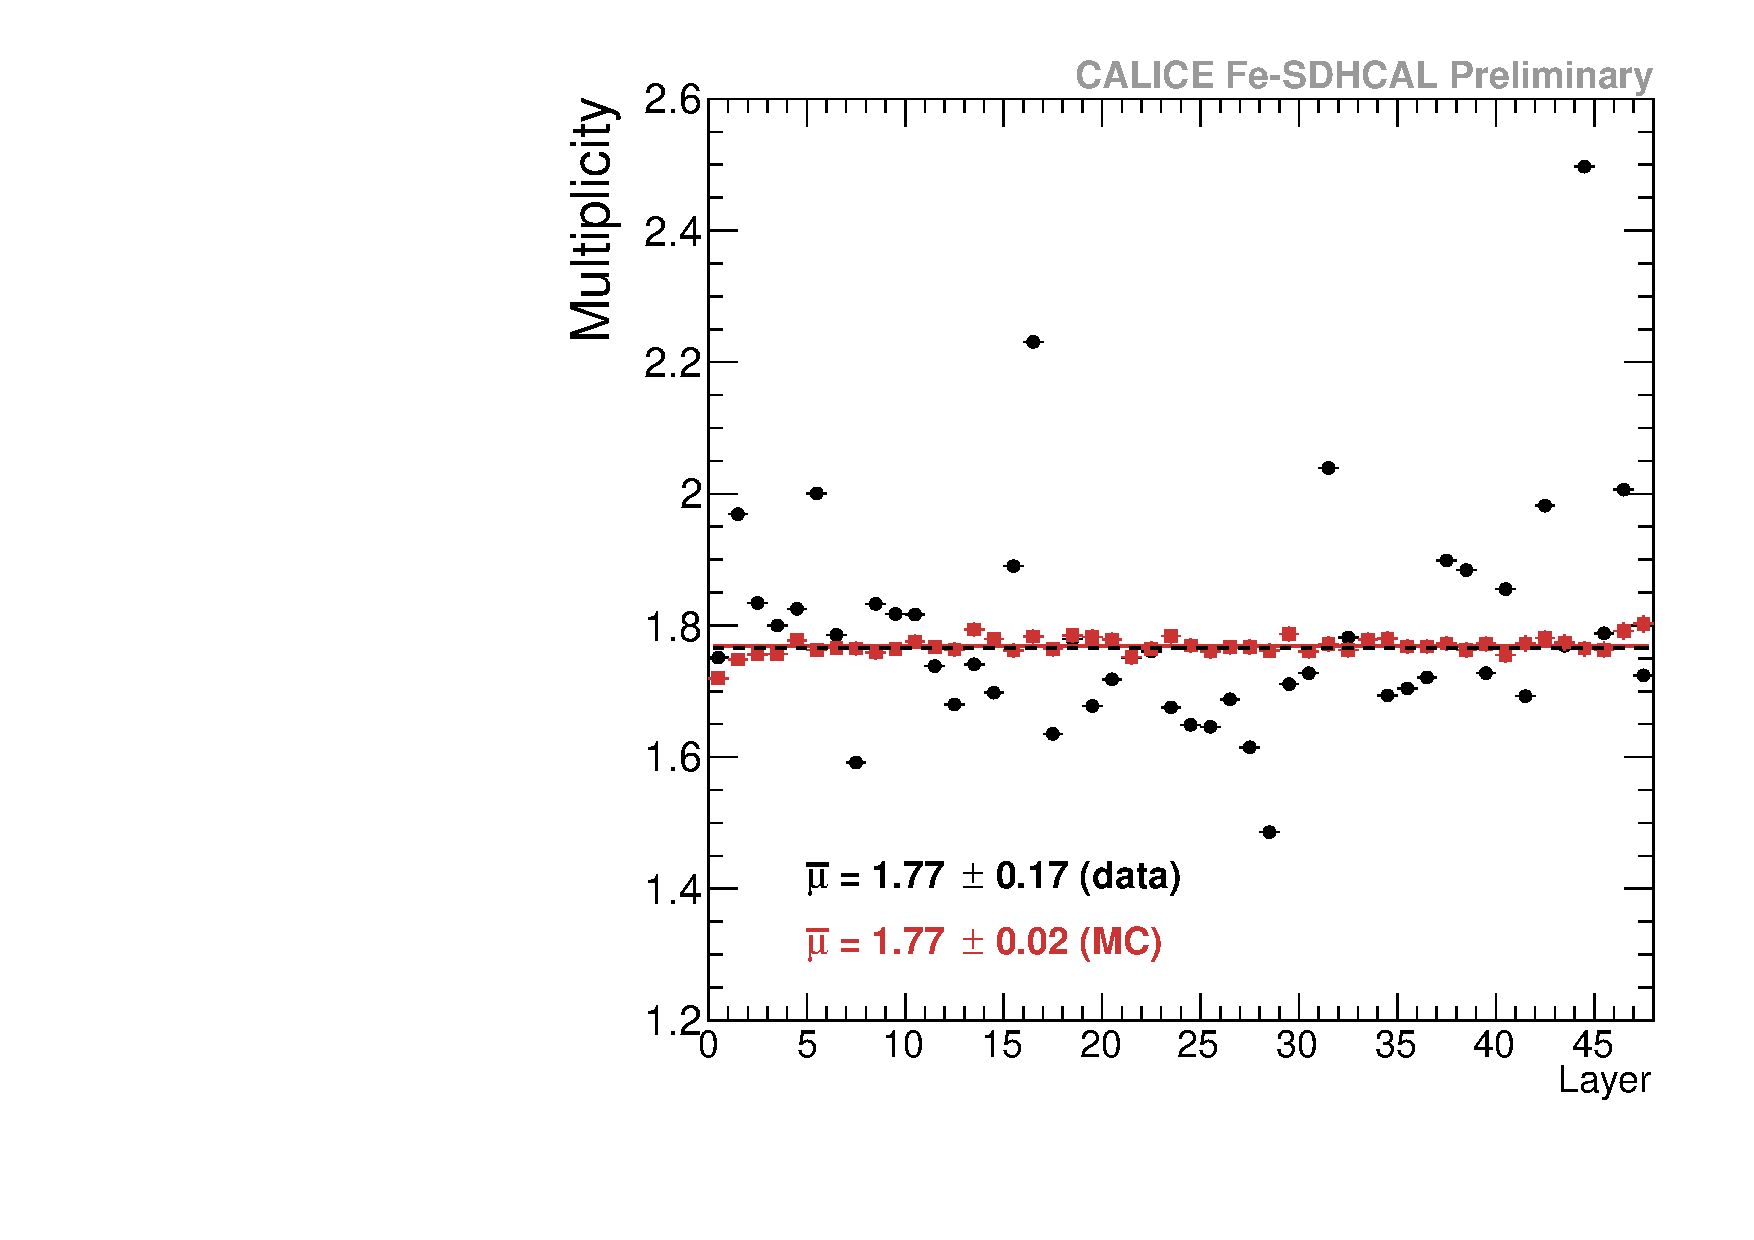
\includegraphics[width=.5\textwidth]{Digitizer/figs/mulLayer.pdf}}
  \caption{Efficacité (a) et multiplicité (b) par plan. Les données sont représentées par des cercles noirs et la simulation par des carrés rouges.\label{fig.eff_mul_layer}}
\end{figure}
L'efficacité dans la simulation suit raisonnablement bien les fluctuations des données car les cartes d'efficacités (déterminés avec les données) sont utilisés par l'algorithme. En revanche, les fluctuations de multiplicité ne sont pas reproduite par la simulation. Les différences de multiplicité d'une chambre à l'autre peuvent s'expliquer par des différences de résistivité de la peinture appliquée sur les verres et par des imperfections de la géométrie des détecteurs.
%%%%%%%%%%%%%%%%%%%%%%%%%%%%%%%%%%%%%

\subsubsection{Dépendance de l'angle d'incidence}
Lors des tests sur faisceau, les muons incidents sont pour la plupart perpendiculaires au detecteurs. Cependant, dans les gerbes hadroniques et électromagnétiques des particules secondaires sont émises avec des angles différents. Une étude de la multiplicité avec des particules cosmiques est alors nécessaire pour déterminer et simuler la réponse d'une GRPC sur une large gamme d'angle d'incidences. La figure~\ref{fig.mul_vs_theta}(a) montre la multiplicité en fonction de $cos{\theta}$ où $\theta$ est angle entre la normale au détecteur et la particule incidente. Cette figure montre que la multiplicité pour les données expérimentales, augmente avec l'angle de la particule incidente alors qu'elle est plus plate pour la simulation. Une correction de la charge simulée est nécessaire pour reproduire le comportement des données. Une correction utilisant l'équation~\ref{eq.lengthcorrection} est préférée à une correction utilisant "$\frac{1}{cos\theta'}$" (avec $\theta'$ l'angle entre le segment et la normale au détecteur) car cette dernière peut générer des charges simulées infinies. 
\begin{figure}[!ht]
  \subfigure[]{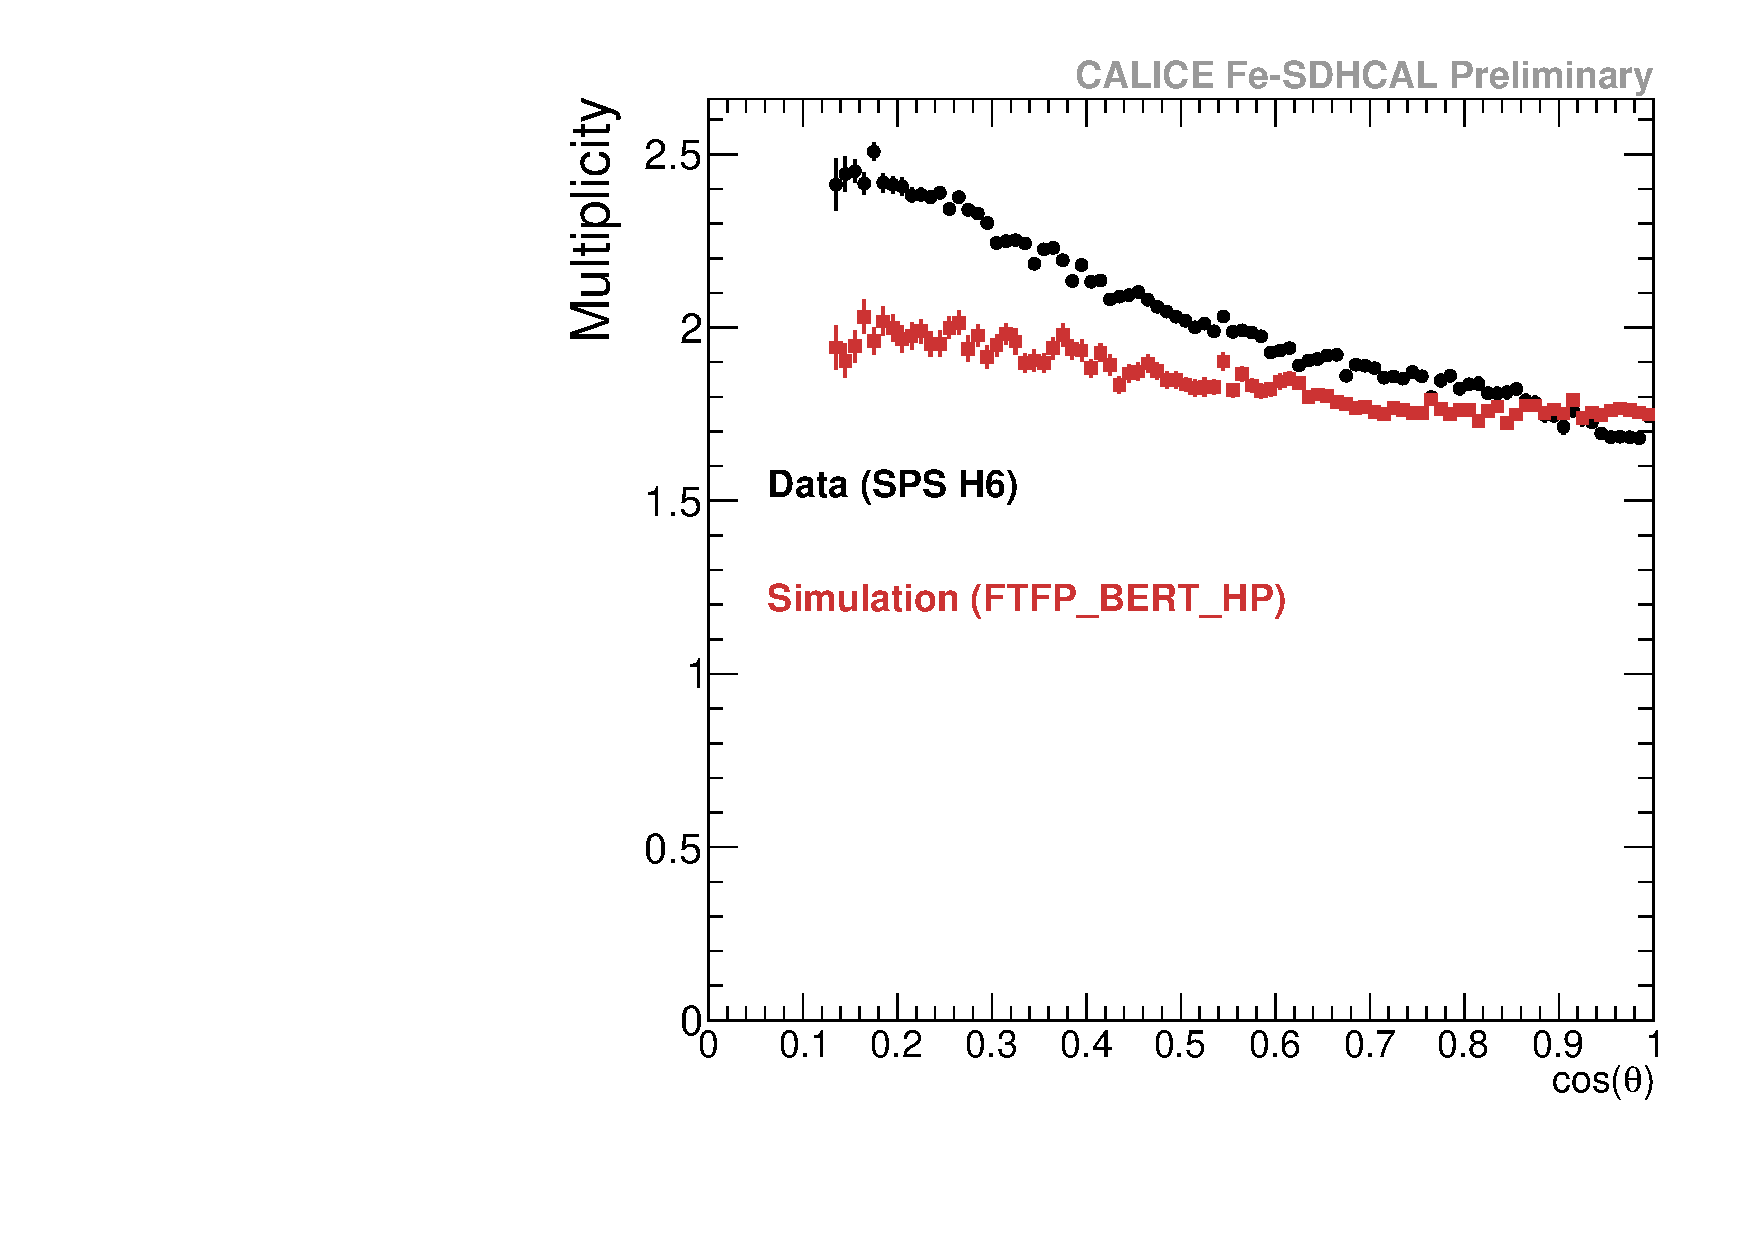
\includegraphics[width=.5\textwidth]{Digitizer/figs/mul_vs_thetaNLC.pdf}}
  \subfigure[]{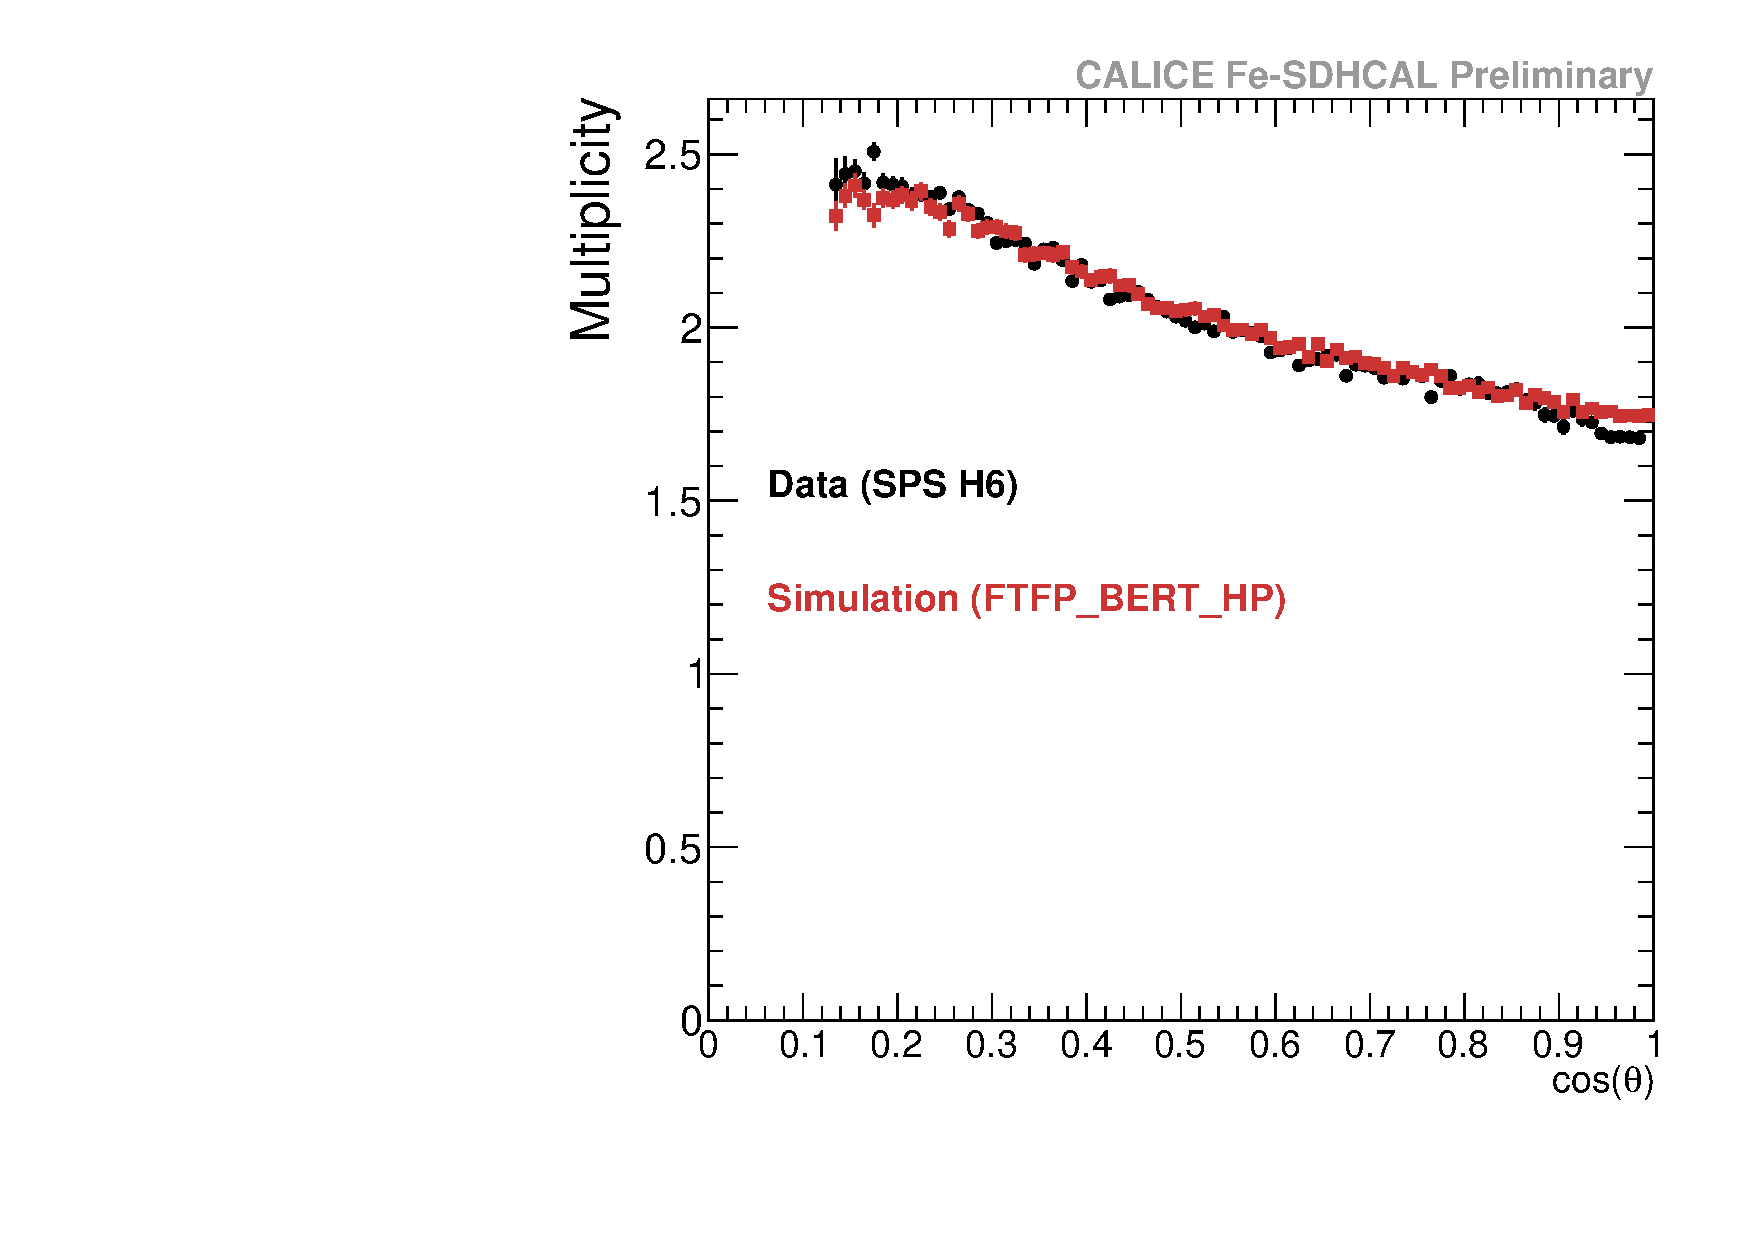
\includegraphics[width=.5\textwidth]{Digitizer/figs/mul_vs_theta.pdf}}
  \caption{Multiplicité moyenne en fonction de $cos\theta$ avec des cercles noirs et des carré rouges pour les données et la simulation respectivement. (a): sans correction sur la longueur des steps; (b) avec correction sur la longueur des steps. \label{fig.mul_vs_theta}}
\end{figure}
La figure~\ref{fig.mul_vs_theta}(b) montre un bon accord entre les données et la simulation pour la multiplicité en fonction de $cos\theta$ après l'application de cette correction. La valeur du facteur $\kappa$ est fixée à 0.33.
%% \begin{figure}[!ht]
%%   \begin{center}
%%     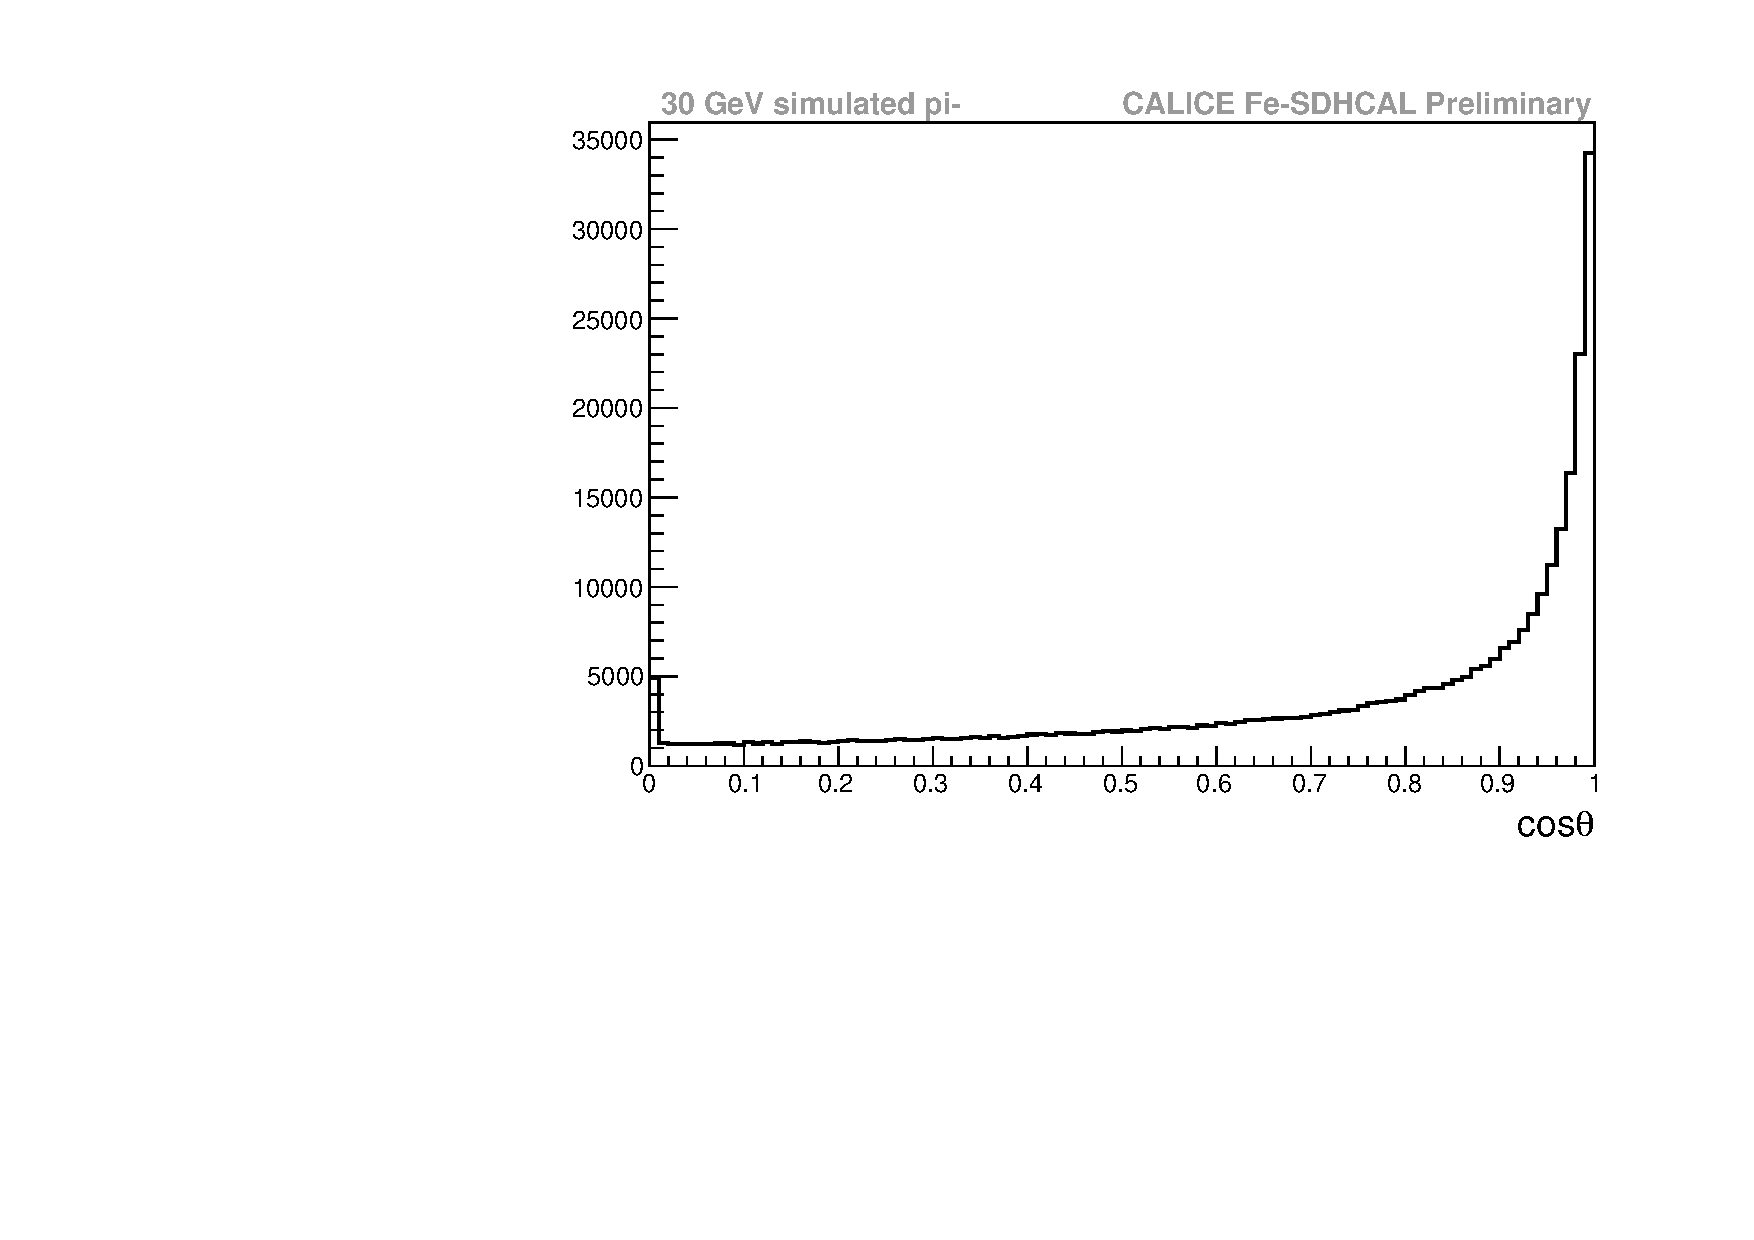
\includegraphics[width=.8\textwidth]{Digitizer/figs/costhetaPI30.pdf}
%%     \caption{Distribution du cos de l'angle de la step avec la normal à la GRPC pour une simulation d'un échantillon de pion à 30 GeV.}
%%     \label{fig.g4list}
%%   \end{center}
%% \end{figure}

%%%%%%%%%%%%%%%%%%%%%%%%%%%%%%%%%%%%%

\subsubsection{Paramétrisation des seuils}
Nous avons vu dans la setion~\ref{sec.sdhcal_thr} du chapitre~\ref{chap.sdhcal} comment les seuils étaient réglés dans le prototype. Cependant comme ces travaux n'ont pas pu être effectuer avec des détecteurs complet, il est probable que les valeurs de conversion (entre DAC et valeurs de seuil en $pC$) soient légèrement différentes pour le prototype. Ceci donne un peu de liberté pour régler les seuils dans la simulation. La figure~\ref{fig.thrScan}(b) montre qu'une faible variation du premier seuil ($seuil\in[0.1,0.4]~pC$) a des conséquences négligeable sur l'efficacité ($\varepsilon\in[0.94,0.95]$). Ainsi, la valeur du premier seuil utilisé dans la simulation est calculé avec l'équation~\ref{eq.dacConversion}. Pour régler la valeur des seuils supérieur, nous avons de nouveau réalisé une étude d'efficacité. La même méthode décrite dans la partie~\ref{sec.polya} est utilisé pour déterminer si un plan est efficace. Lorsqu'un plan est efficace, il est aussi considéré comme efficace pour les seuils 2 et/ou 3 si au moins un coups ayant passé ces seuils sont trouvés dans le groupe de coups correspondant. Les seuils 2 et 3 sont alors régler pour reproduire les efficacités des données expérimentales. 
\begin{figure}[!ht]
  \subfigure[]{\includegraphics[width=.5\textwidth]{Digitizer/figs/eff2Layer.pdf}}
  \subfigure[]{\includegraphics[width=.5\textwidth]{Digitizer/figs/eff3Layer.pdf}}
  \caption{Efficacité pour le deuxième (a) et le troisième (b) seuil par plan. Les données sont représentées par des cercles noirs et la simulation par des carrés rouges.\label{fig.eff_thr}}
\end{figure}
La figure~\ref{fig.eff_thr} montre les efficacités par plan pour les seuils 2~(fig.~\ref{fig.eff_thr}(a)) et 3~(fig.~\ref{fig.eff_thr}(b)) pour la simulation et pour les données. Les seuils 2 et 3 sont fixés à 5.4 et 14.0 $pC$ respectivement pour la simulation alors que pour les données l'équation~\ref{eq.dacConversion} indique des valeurs de seuils de 5.0 et 15.0 $pC$~($DAC_2=500$; $DAC_3=345$).
%%%%%%%%%%%%%%%%%%%%%%%%%%%%%%%%%%%%%

\subsubsection{Résumé}
La valeur de deux paramètres n'a pas été encore discuté. Le paramètre $l_{min}$ est fixé à 1 $\mu m$. Nous avons vérifié que l'effet de petite variation autour de cette valeur est négligeable. Le paramètre $d_{cut}$ est fixé à 1 $mm$. Il a été régler pour reproduire le nombre de coups dans les gerbes électromagnétiques (c.f. section~\ref{sec.resultats}). Le tableau~\ref{tab.summary} contient la liste des paramètres introduits dans l'algorithme et leur valeur.
\begin{table}[!ht]
  \begin{center}
    \begin{tabular}{c||c}
      Paramètre & Valeur \\
      \hline
      \hline
      $l_{min}$ & $0.001\ mm$\\
      $d_{cut}$ & $1\ mm$ \\
      \hline
      $\bar q$ & $4.53\ pC$ \\
      $\theta$ & $1.05$ \\ 
      \hline
      $n$ & $2$ \\ 
      $r_{max}$ & $30\ mm$ \\
      $\alpha_0$ & $1.0$ \\
      $\sigma_0$ & $1.0\ mm$ \\
      $\alpha_1$ & $0.00083$ \\
      $\sigma_1$ & $9.7\ mm$ \\
      \hline
      $\kappa$ & $0.33$\\
      \hline 
      $seuil_1$ & $0.114\ pC$\\
      $seuil_2$ & $5.4\ pC$\\
      $seuil_3$ & $14\ pC$
    \end{tabular}
  \end{center}  
  \caption{Paramètres d'entrée de l'algorithme SimDigital.}
  \label{tab.summary}
\end{table}
%%%%%%%%%%%%%%%%%%%%%%%%%%%%%%%%%%%%%

\subsection{Résultats}
\label{sec.resultats}
Nous avons vu les différentes méthodes utilisées pour régler les valeurs des paramètres introduits dans l'algorithme SimDigital. Nous allons maintenant tester cet algorithme avec des gerbes électromagnétiques puis hadroniques. Dans cette section, les mêmes coupures sont appliquées sur les échantillons de données pour filtrer les muons du faisceaux, les particules cosmiques et les particules neutres que dans la section~\ref{sec.shower_selection} du chapitre~\ref{chap.sdhcal}. La différenciation des gerbes électromagnétiques et hadroniques sera décrites dans les sous parties correspondantes. Les coupures appliquées aux données expérimentales sont aussi appliquées sur les échantillons de simulation afin d'éviter des biais. Les listes physiques utilisées dans la suite sont FTFP\_BERT\_HP et QGSP\_BERT\_HP. Enfin, rappelons que le nombre de coups dans les gerbes est calibré avec le temps (voir section~\ref{sec.timeCalib} du chapitre~\ref{chap.sdhcal}).

%%%%%%%%%%%%%%%%%%%%%

\subsubsection{Gerbes électromagnétique}
 Les gerbes électromagnétiques sont traditionnellement bien simulées par GEANT4. Les comparaisons entre les données expérimentales et la simulation des gerbes électromagnétiques n'auront pas pour objectif de valider ou d'invalider les modèles de GEANT4 mais plutôt de vérifier la qualité de l'algorithme introduit pour modéliser la réponse des GRPCs au passage de particules chargées. De plus certains paramètres de l’algorithme ont été réglé pour reproduire la réponse du détecteur lors du passage d'une gerbe électromagnétique.
Pour décider si une gerbe a été induite par un électron, les trois critères suivant doivent être vérifié:
\begin{enumerate}[~~1-]
\item Le nombre de plan avec au moins 1 coup doit être inférieur à 30 (fig.~\ref{fig.e-_begin_layer}(a)).
\item Le nombre de traces reconstruites avec la technique de Transformée de Hough (voir section~\ref{sec.hough} du chapitre~\ref{chap.topo}) 
doit être nulle. %\textcolor{red}{(!!!référence au chapitre sur les topo quand il sera écrit!!!)}
\item Le premier plan d’interaction doit être compris dans un des cinq premiers plans (fig.~\ref{fig.e-_begin_layer}(b)).
  \begin{figure}[!ht]
    \subfigure[]{\includegraphics[width=.5\textwidth]{Digitizer/figs/Nlayer_e-_50GeV.pdf}}
    \subfigure[]{\includegraphics[width=.5\textwidth]{Digitizer/figs/Begin_e-_50GeV.pdf}}
    \caption{(a): Distribution du nombre plans avec au moins un coup pour un échantillon de données de gerbes électromagnétiques à 50 GeV (la coupure sur le nombre de plan n'a pas été appliquée sur cette figure). (b): Distribution du premier plan d’interaction pour un échantillon de données de gerbes électromagnétiques à 50 GeV (la coupure sur le premier plan d'interaction n'a pas été appliquée sur cette figure)\label{fig.e-_begin_layer}}
  \end{figure}
\end{enumerate}

La figure~\ref{fig.e-Selection} montre les distributions de nombre de coups pour des échantillons de données d'électrons à 10 GeV (a) et 50 GeV (GeV) avant les coupures, après les coupures de sélection des électrons et après celles de pions.
\begin{figure}[!ht]
  \subfigure[]{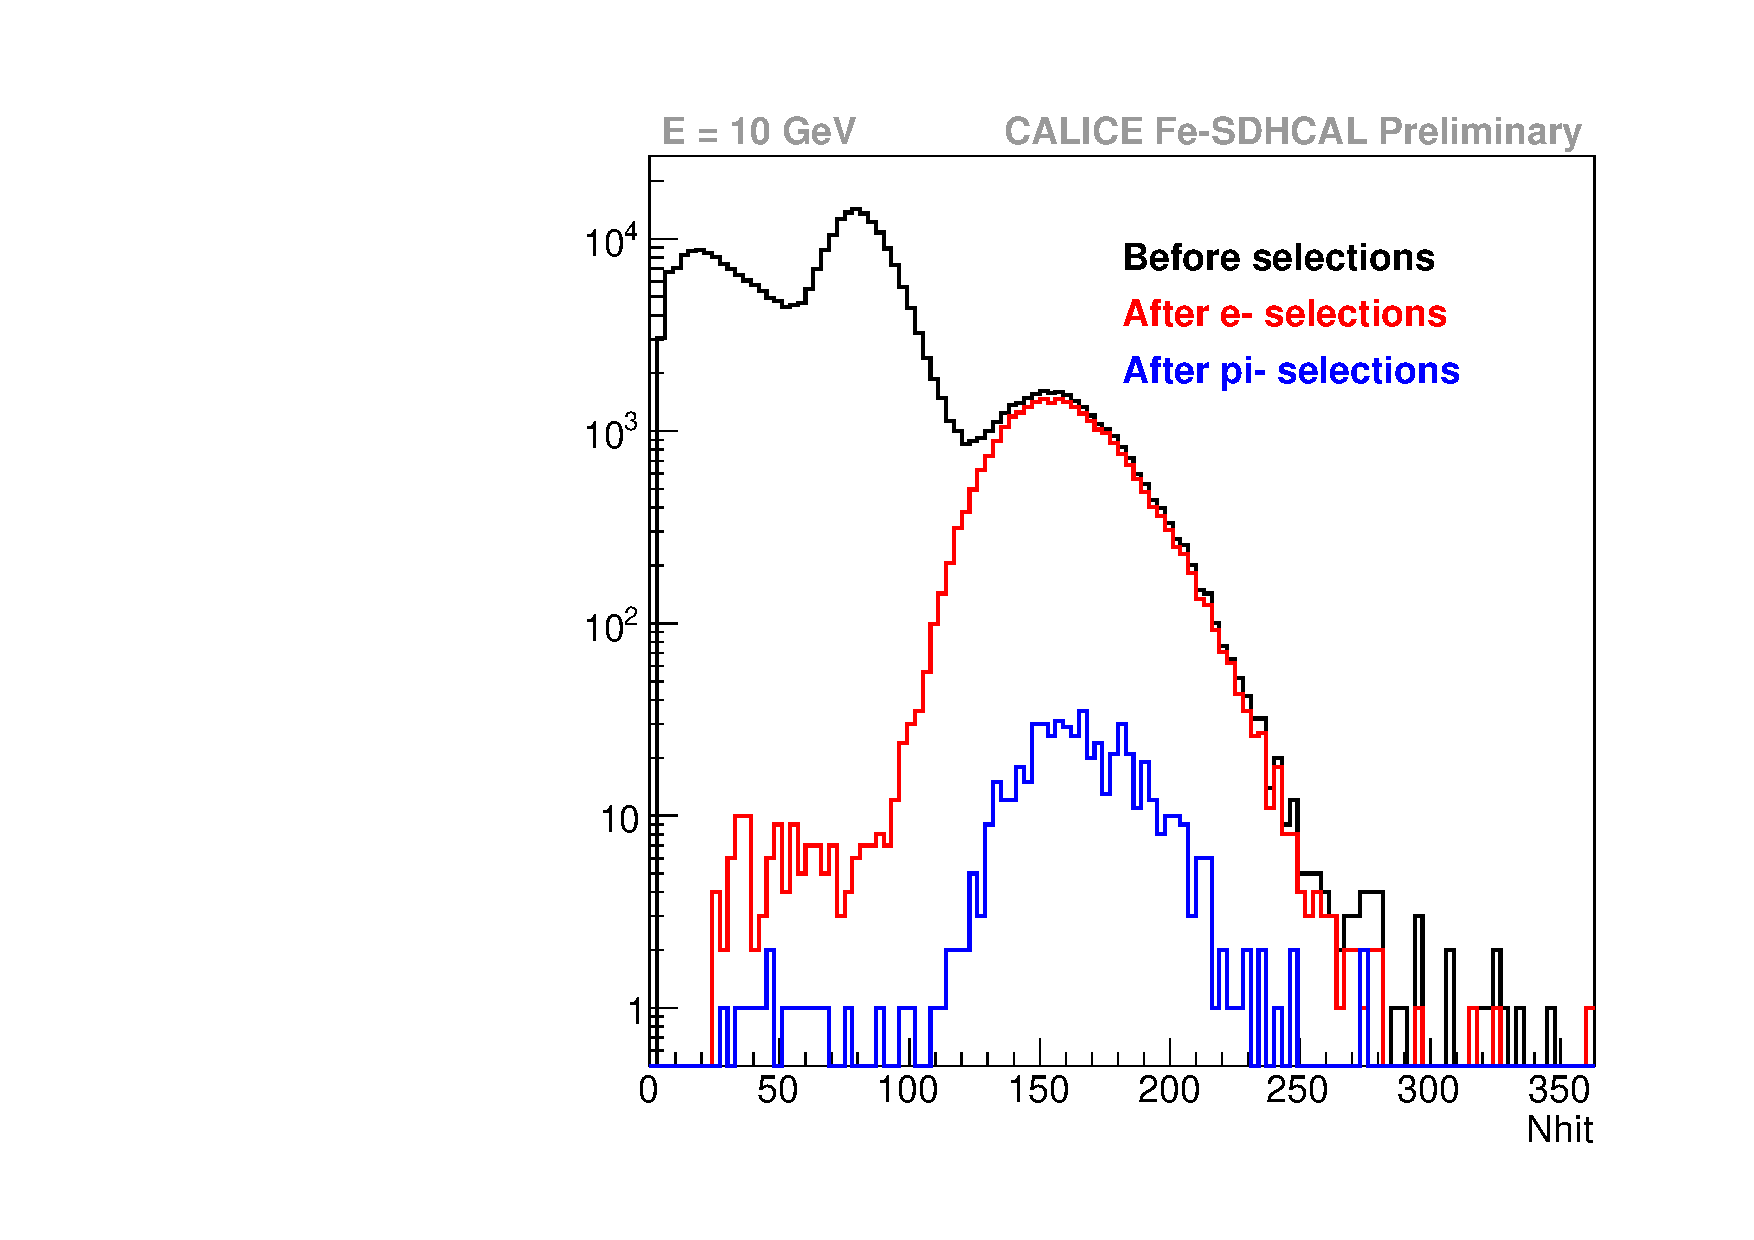
\includegraphics[width=.5\textwidth]{Digitizer/figs/selection715725.pdf}}
  \subfigure[]{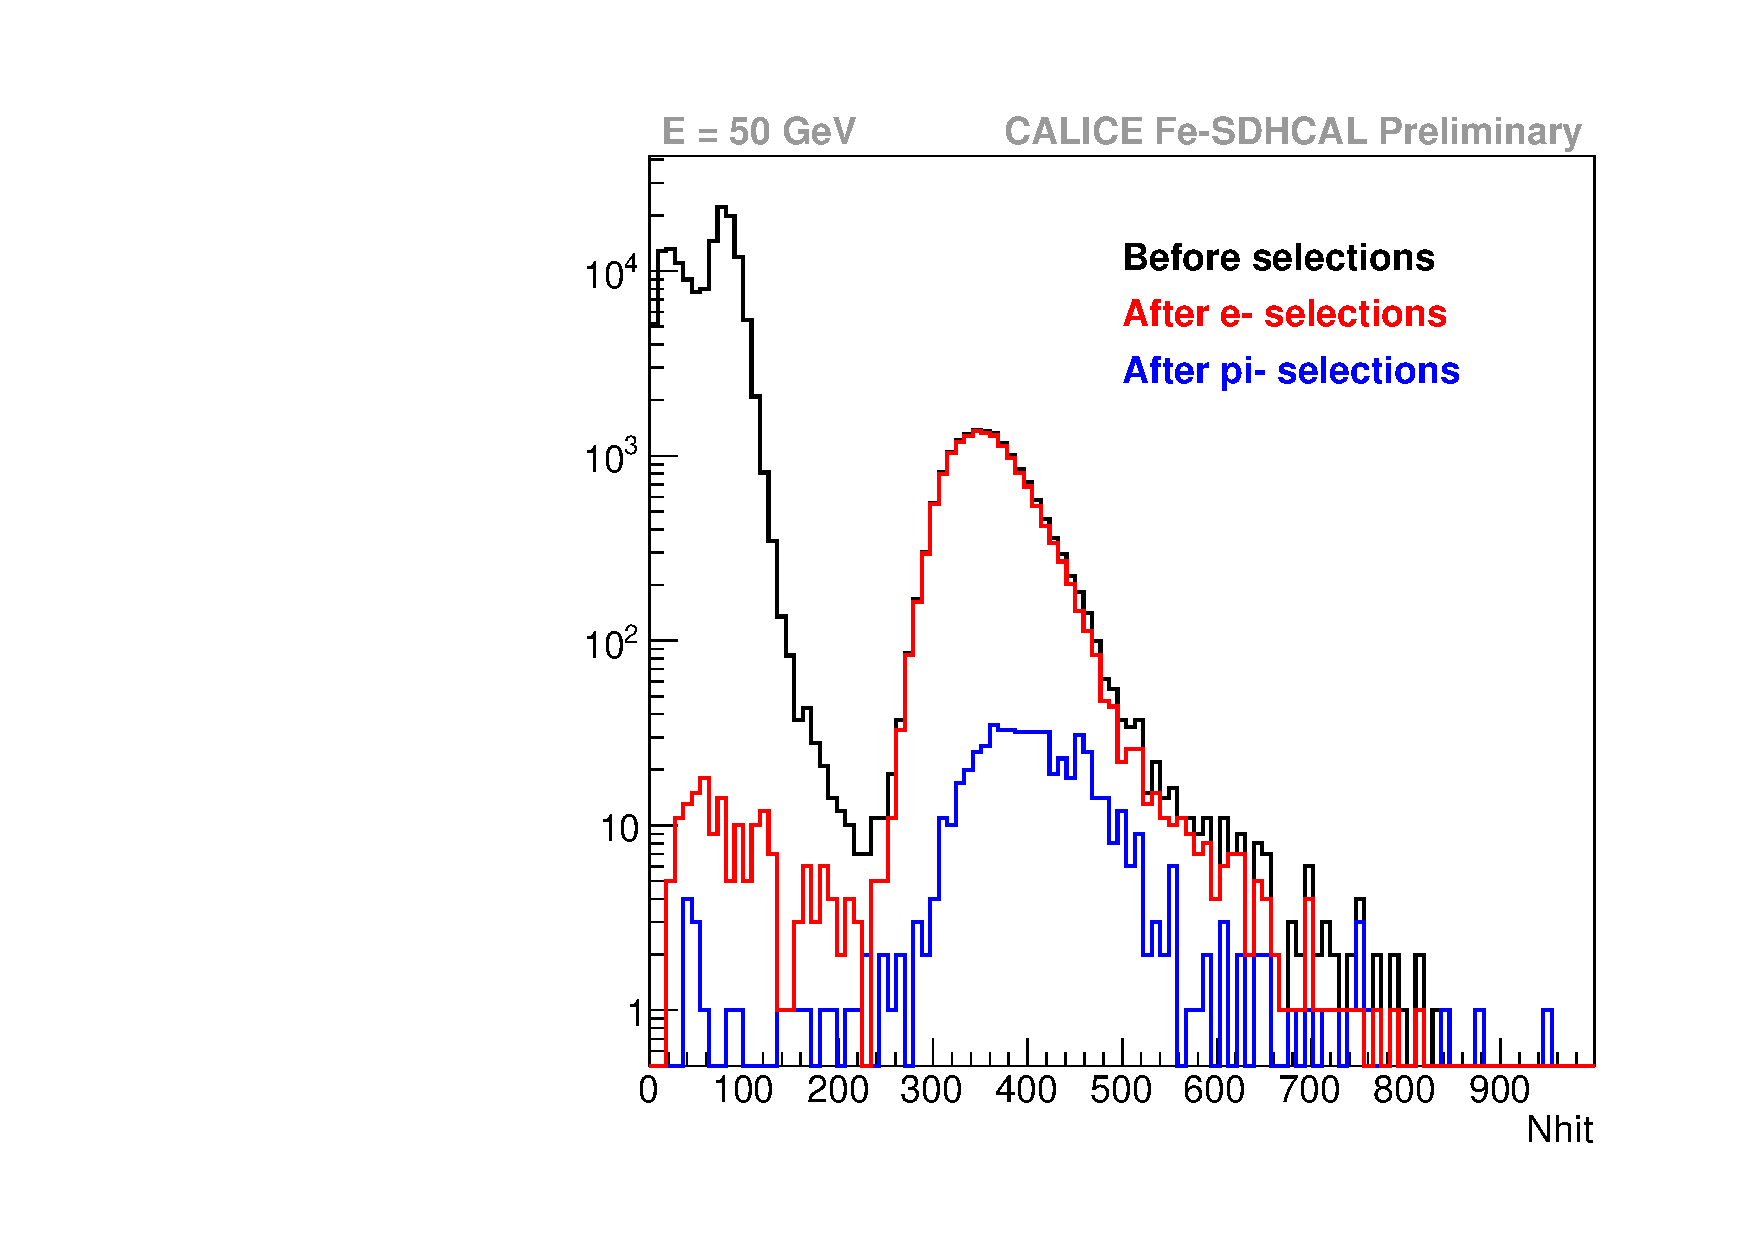
\includegraphics[width=.5\textwidth]{Digitizer/figs/selection715716.pdf}}
  \caption{Distribution du nombre de coups pour des échantillons de données d'électrons à 10 GeV (a) et 50 GeV (GeV). Les lignes noires montrent les distributions de nombres de hits avant les coupures, les lignes rouges après les coupures de sélection des électrons et les lignes bleu après les coupures de sélection des pions. \label{fig.e-Selection}}
\end{figure}

\begin{figure}[!ht]
    \subfigure[]{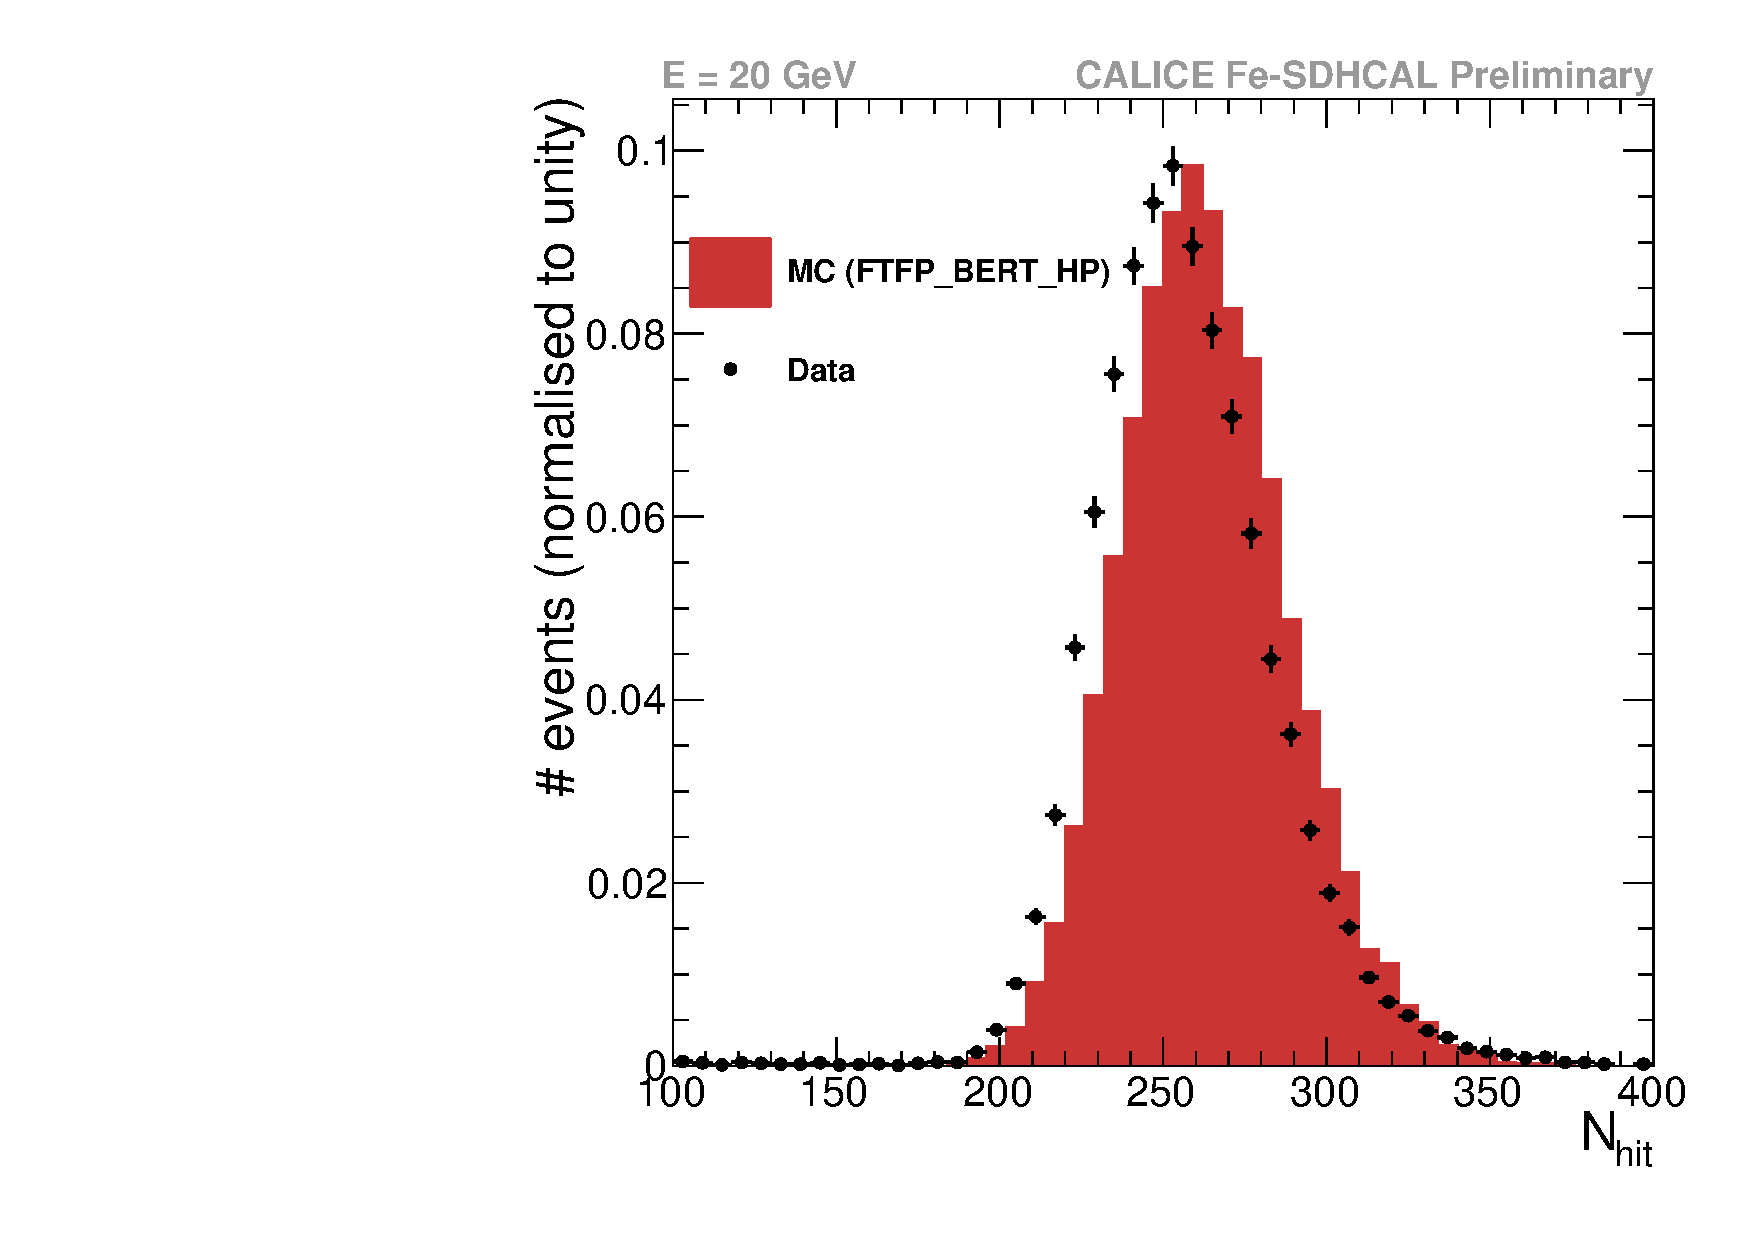
\includegraphics[width=.5\textwidth]{Digitizer/figs/nhit_e-_20GeV_AugSep2012.pdf}}
    \subfigure[]{\includegraphics[width=.5\textwidth]{Digitizer/figs/nhit_e-_50GeV_AugSep2012.pdf}}
    \caption{Distribution de nombre de hits pour des échantillons d'électrons de 20 GeV (a) et 40 GeV (b). Les données sont représenté par des croix noires et la simulation par les histogrammes rouges.}
  \label{fig.nhite-_dist}
\end{figure}
La figure~\ref{fig.nhite-_dist} présente les distributions de nombre de coups pour des échantillons de gerbes électromagnétiques à 20 et 50 $GeV$ pour les données et la simulation. La figure~\ref{fig.nhite-} montre les valeurs moyennes de nombre de coups dans les gerbes électromagnétiques en fonction de l'énergie pour les données et la simulation. Les déviations relatives entre les données et la simultaion définit comme $\frac{N_{hit}^{sim}-N_{hit}^{data}}{N_{hit}^{data}}$ sont aussi indiqués sur cette figure. L'accord entre les données expérimentales et les deux listes physiques utilisées pour la simulation est très satisfaisant. Les déviations relatives sont inférieurs à 3\% sur toute la gamme d'énergie. Ces résultats ont tendance à valider l'algorithme de modélisation et sa paramétrisation. 
\begin{figure}[!ht]
  \centering
  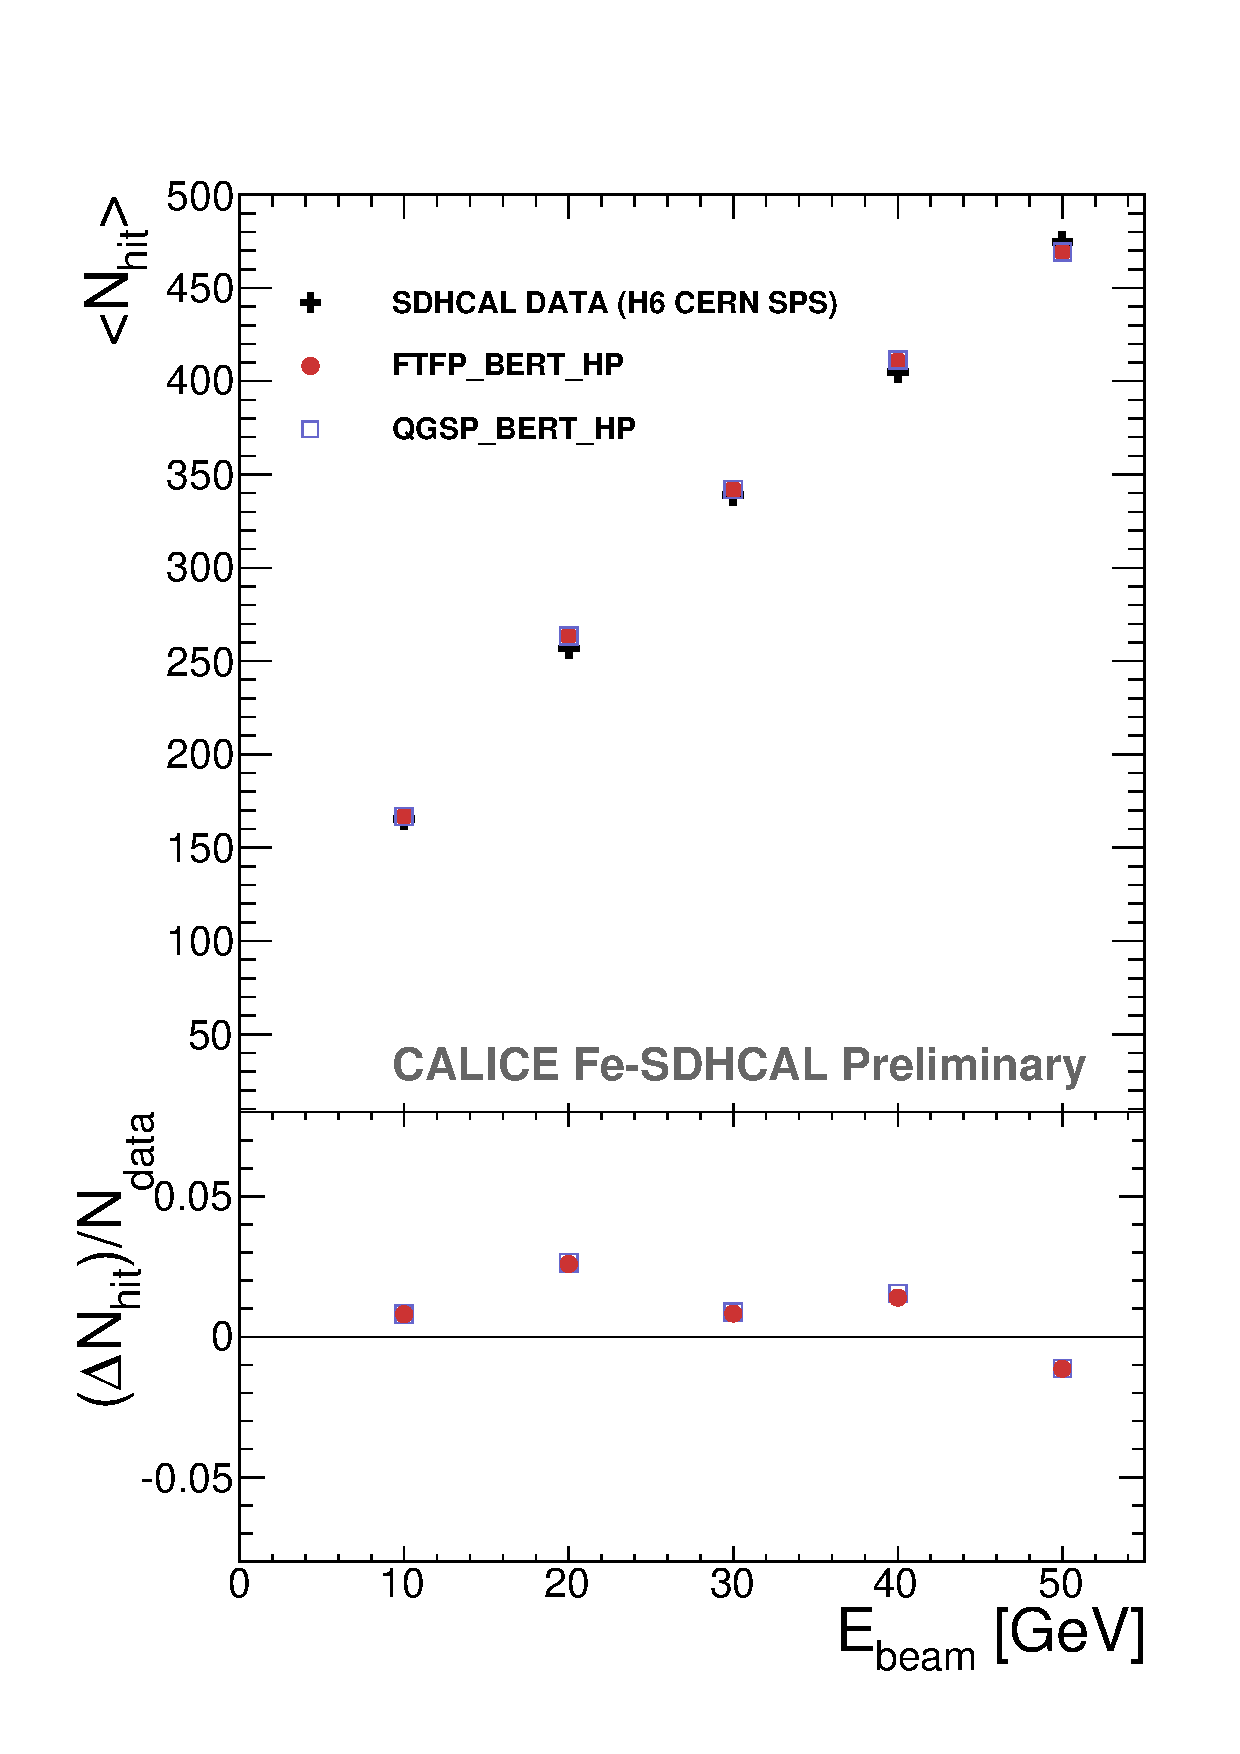
\includegraphics[width=0.5\textwidth]{Digitizer/figs/NHITELECTRON.pdf}
  \caption{(Moyenne du nombre de hits pour des échantillons d'électrons en fonction de l’énergie du faisceau. Les données sont représentés par des croix noires et la simulation par des cercles rouges (FTFP\_BERT\_HP) et des carrés bleus (QGSP\_BERT\_HP). La déviation relative est aussi présentée.}
  \label{fig.nhite-}
\end{figure}

%%%%%%%%%%%%%%%%%%%%%

\subsubsection{Gerbes hadroniques}

\begin{figure}[!ht]
  \subfigure[]{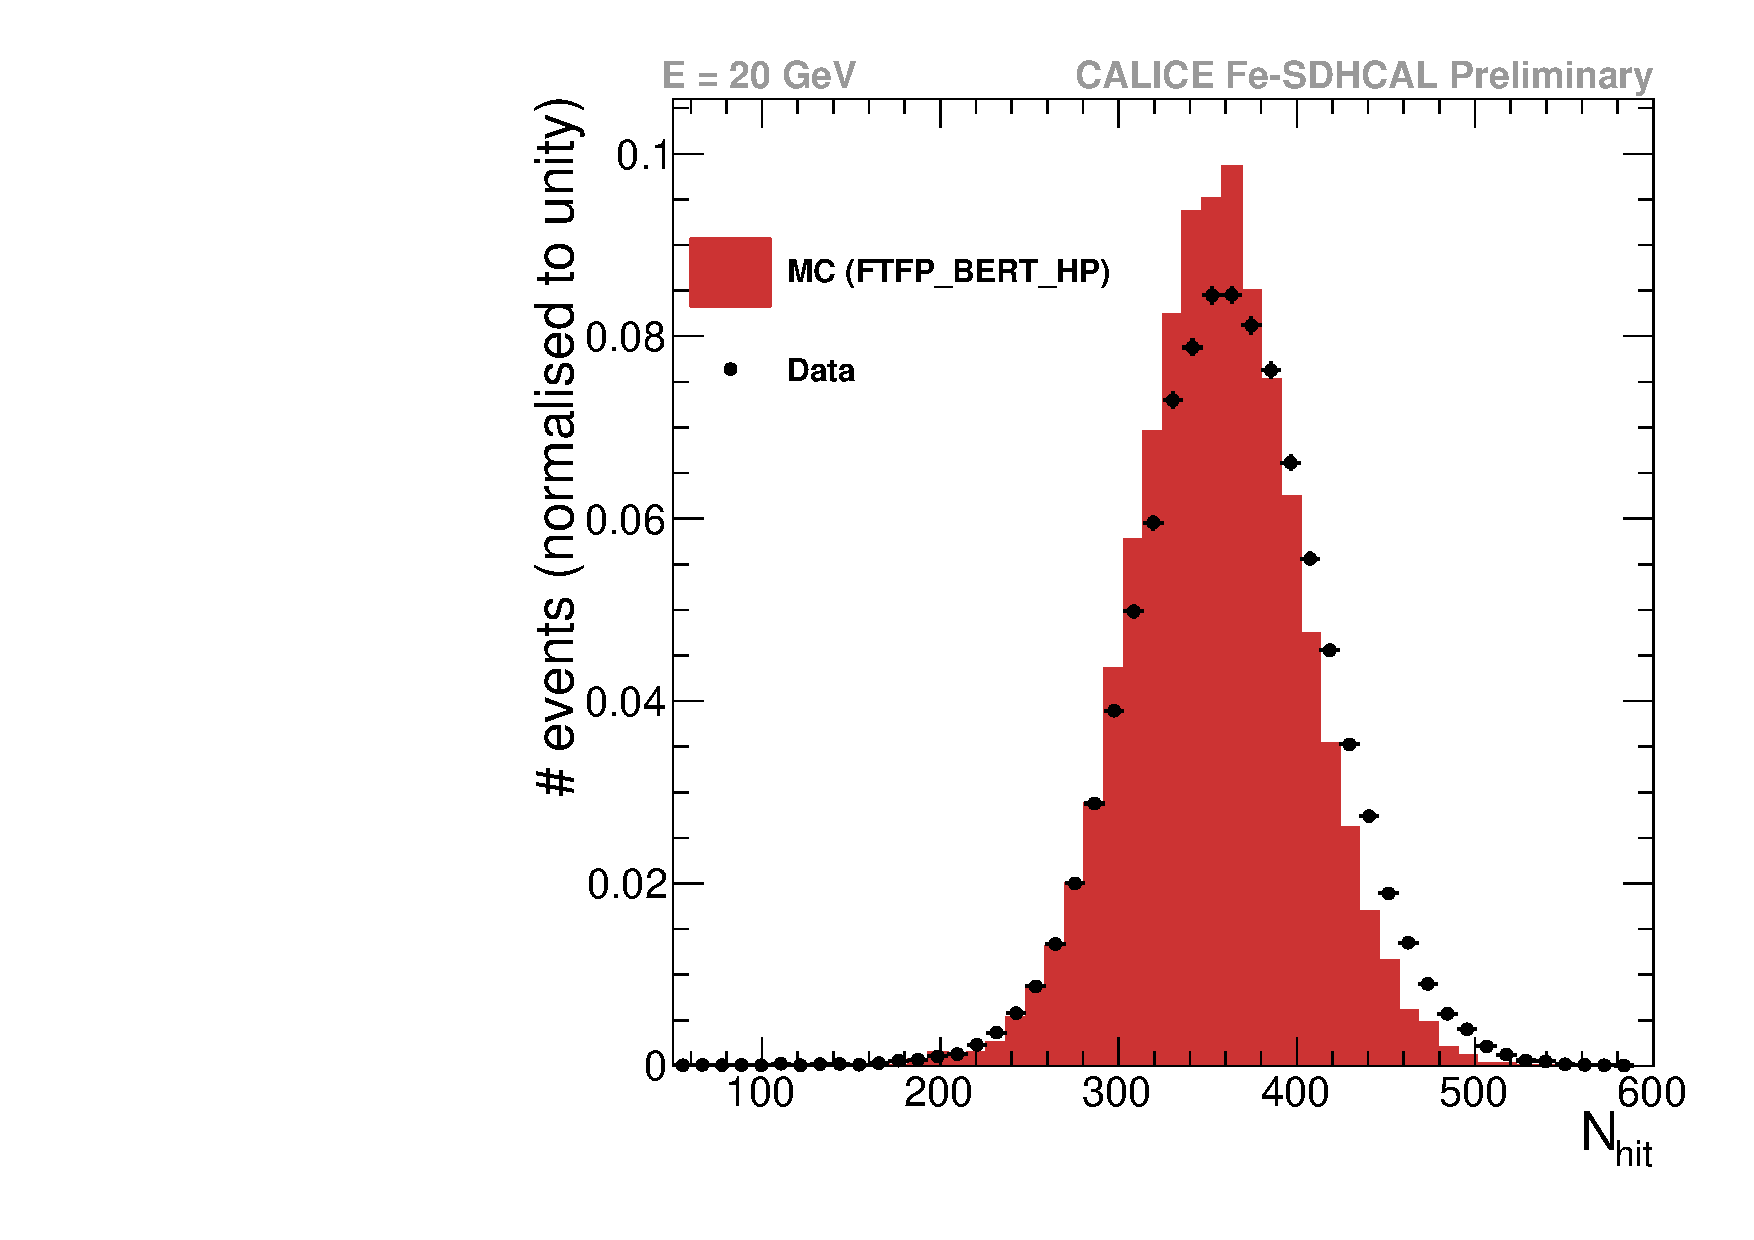
\includegraphics[width=.5\textwidth]{Digitizer/figs/nhit_pi-_20GeV_AugSep2012.pdf}}
  \subfigure[]{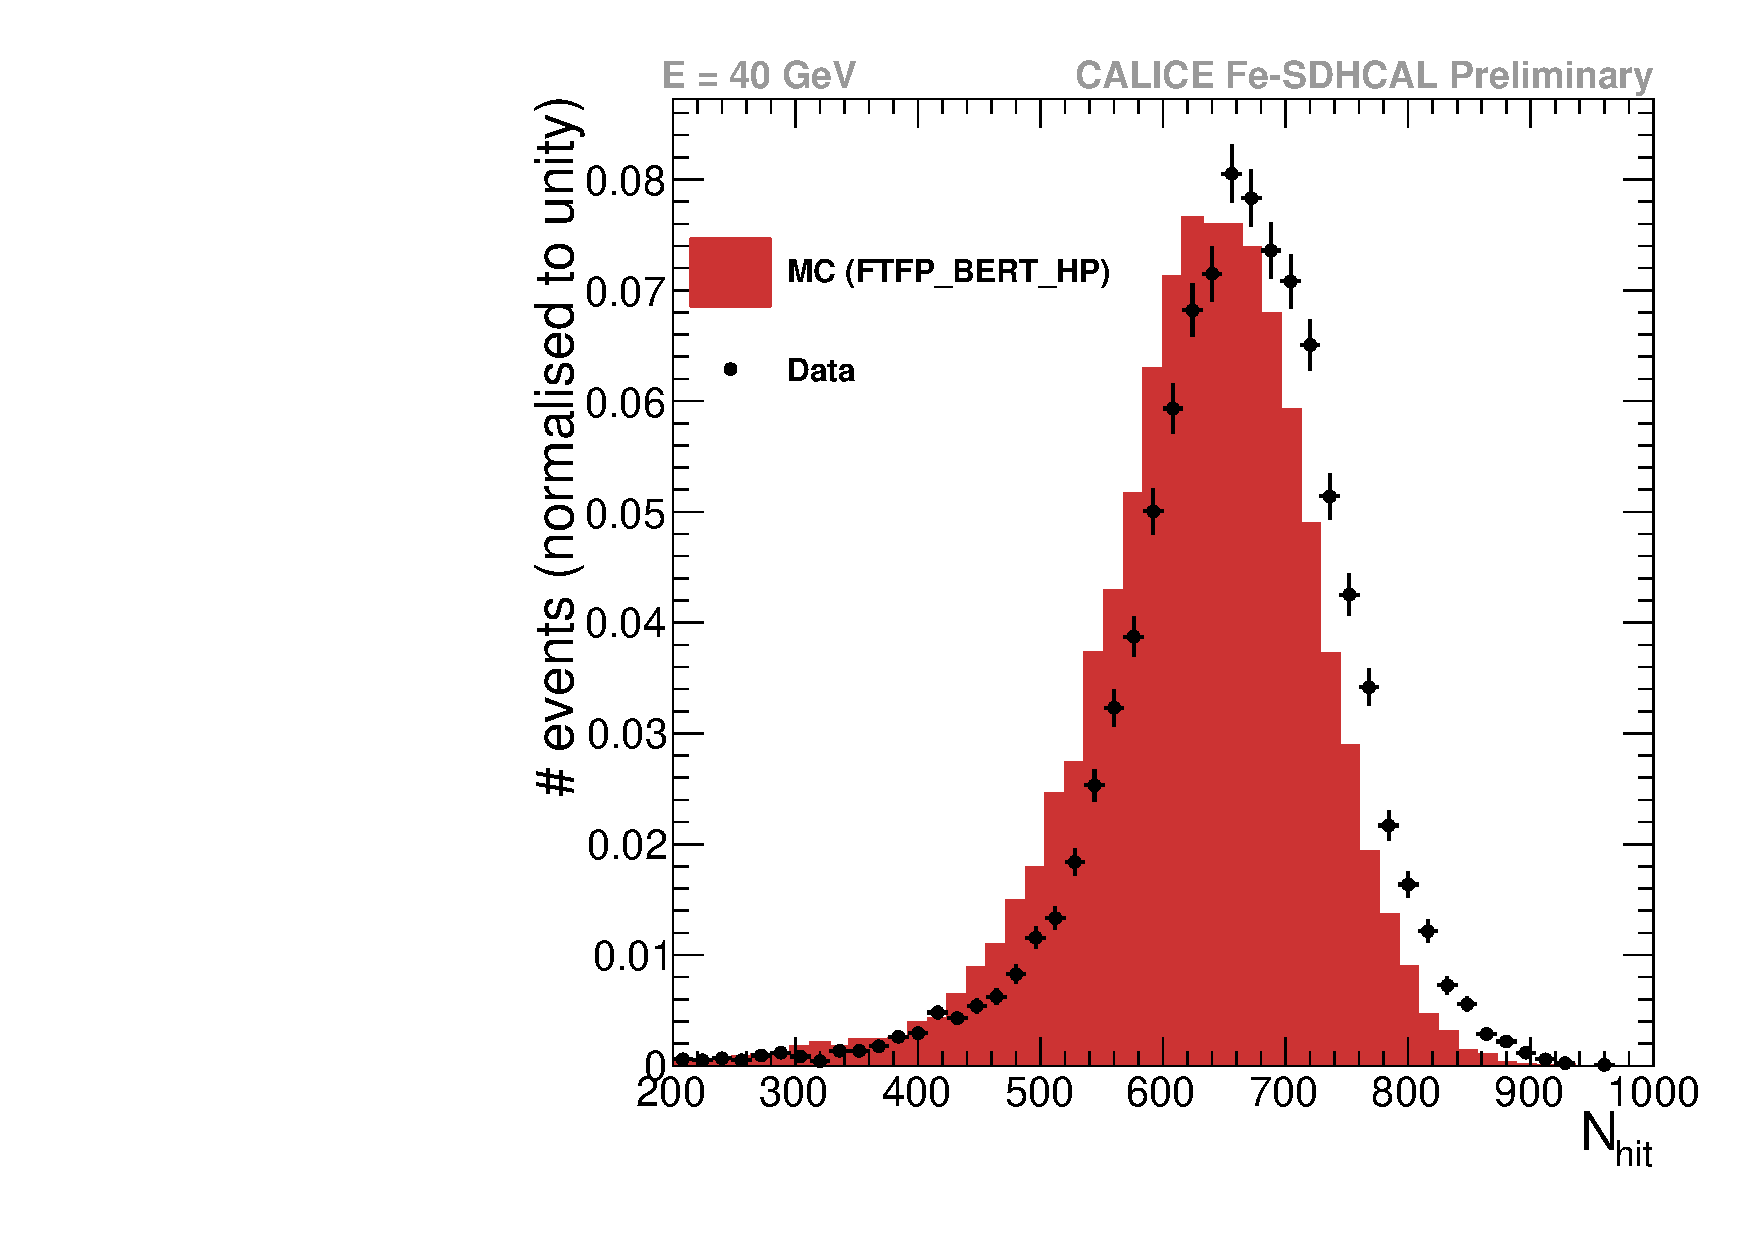
\includegraphics[width=.5\textwidth]{Digitizer/figs/nhit_pi-_40GeV_AugSep2012.pdf}}
  \subfigure[]{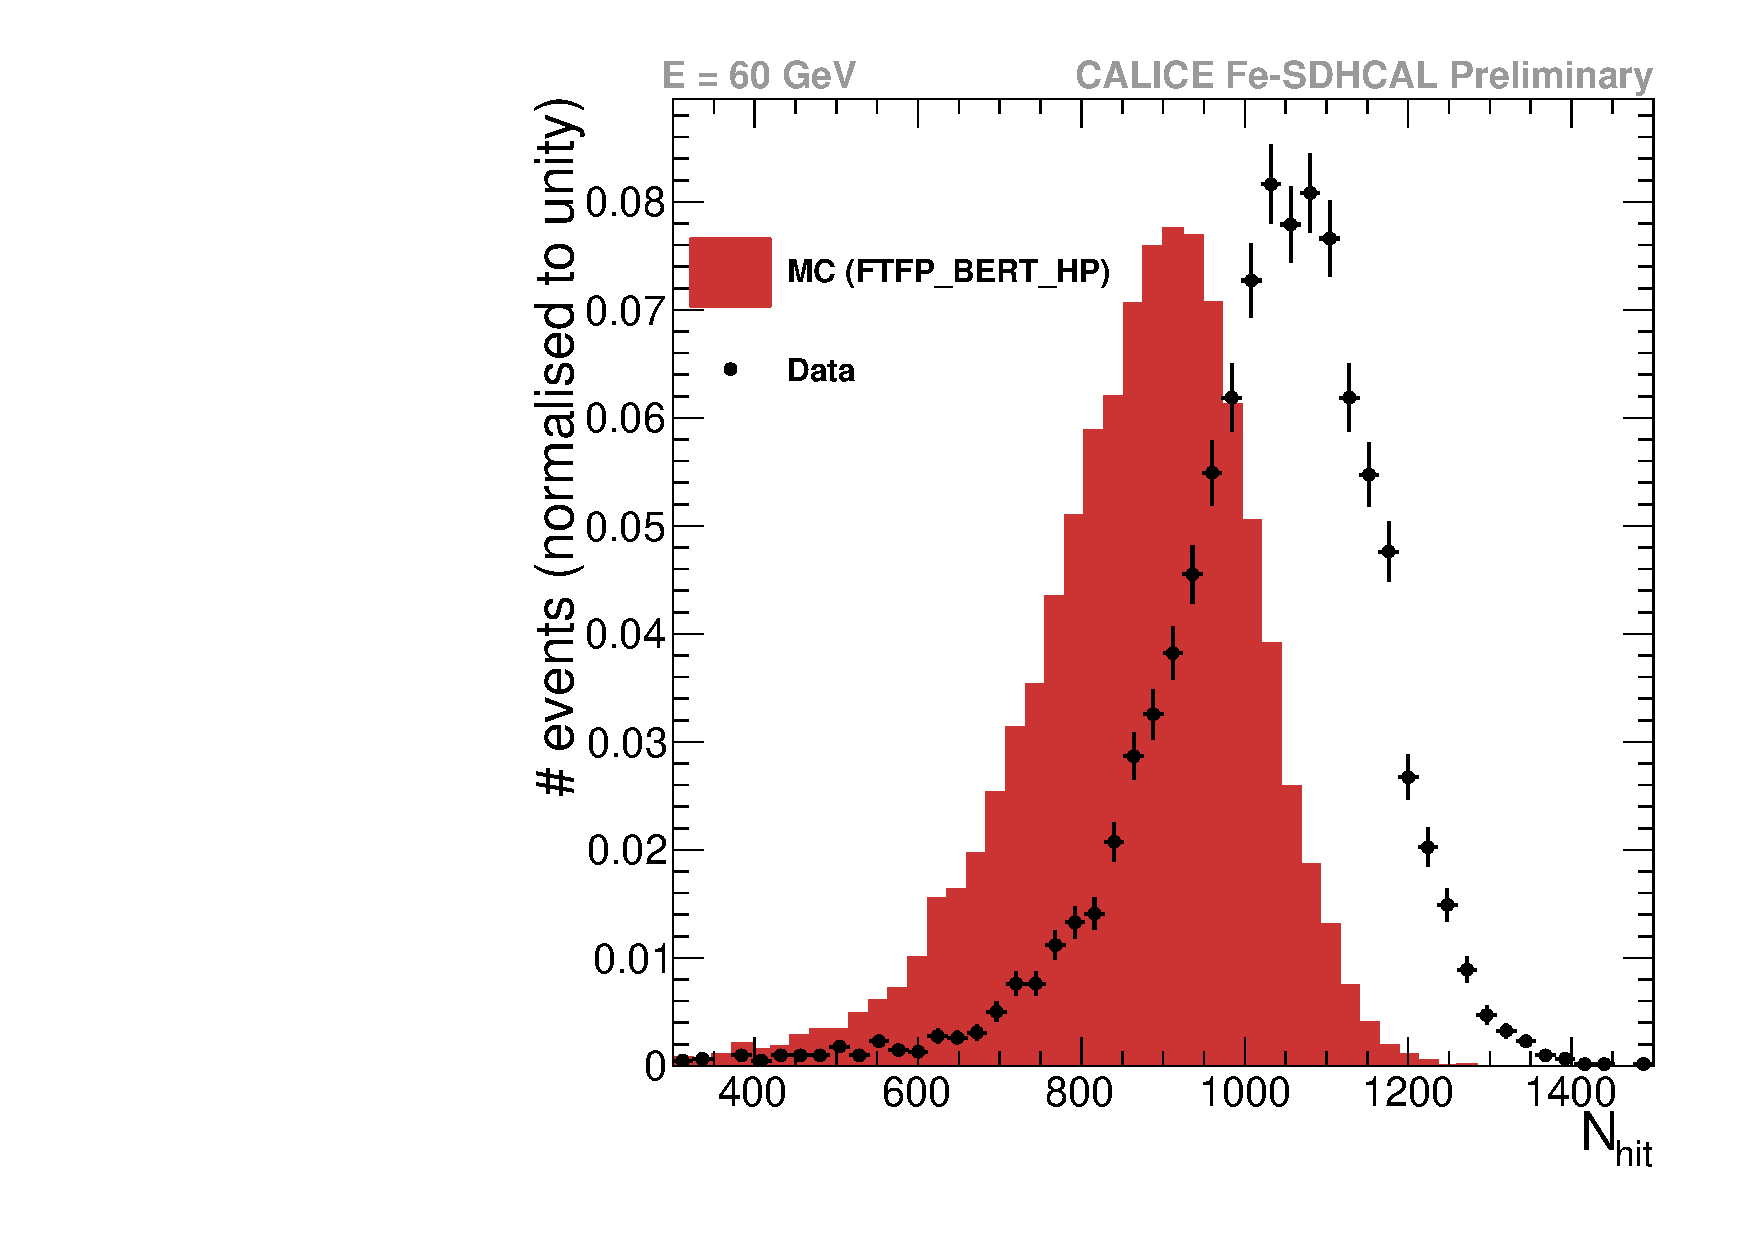
\includegraphics[width=.5\textwidth]{Digitizer/figs/nhit_pi-_60GeV_AugSep2012.pdf}}
  \subfigure[]{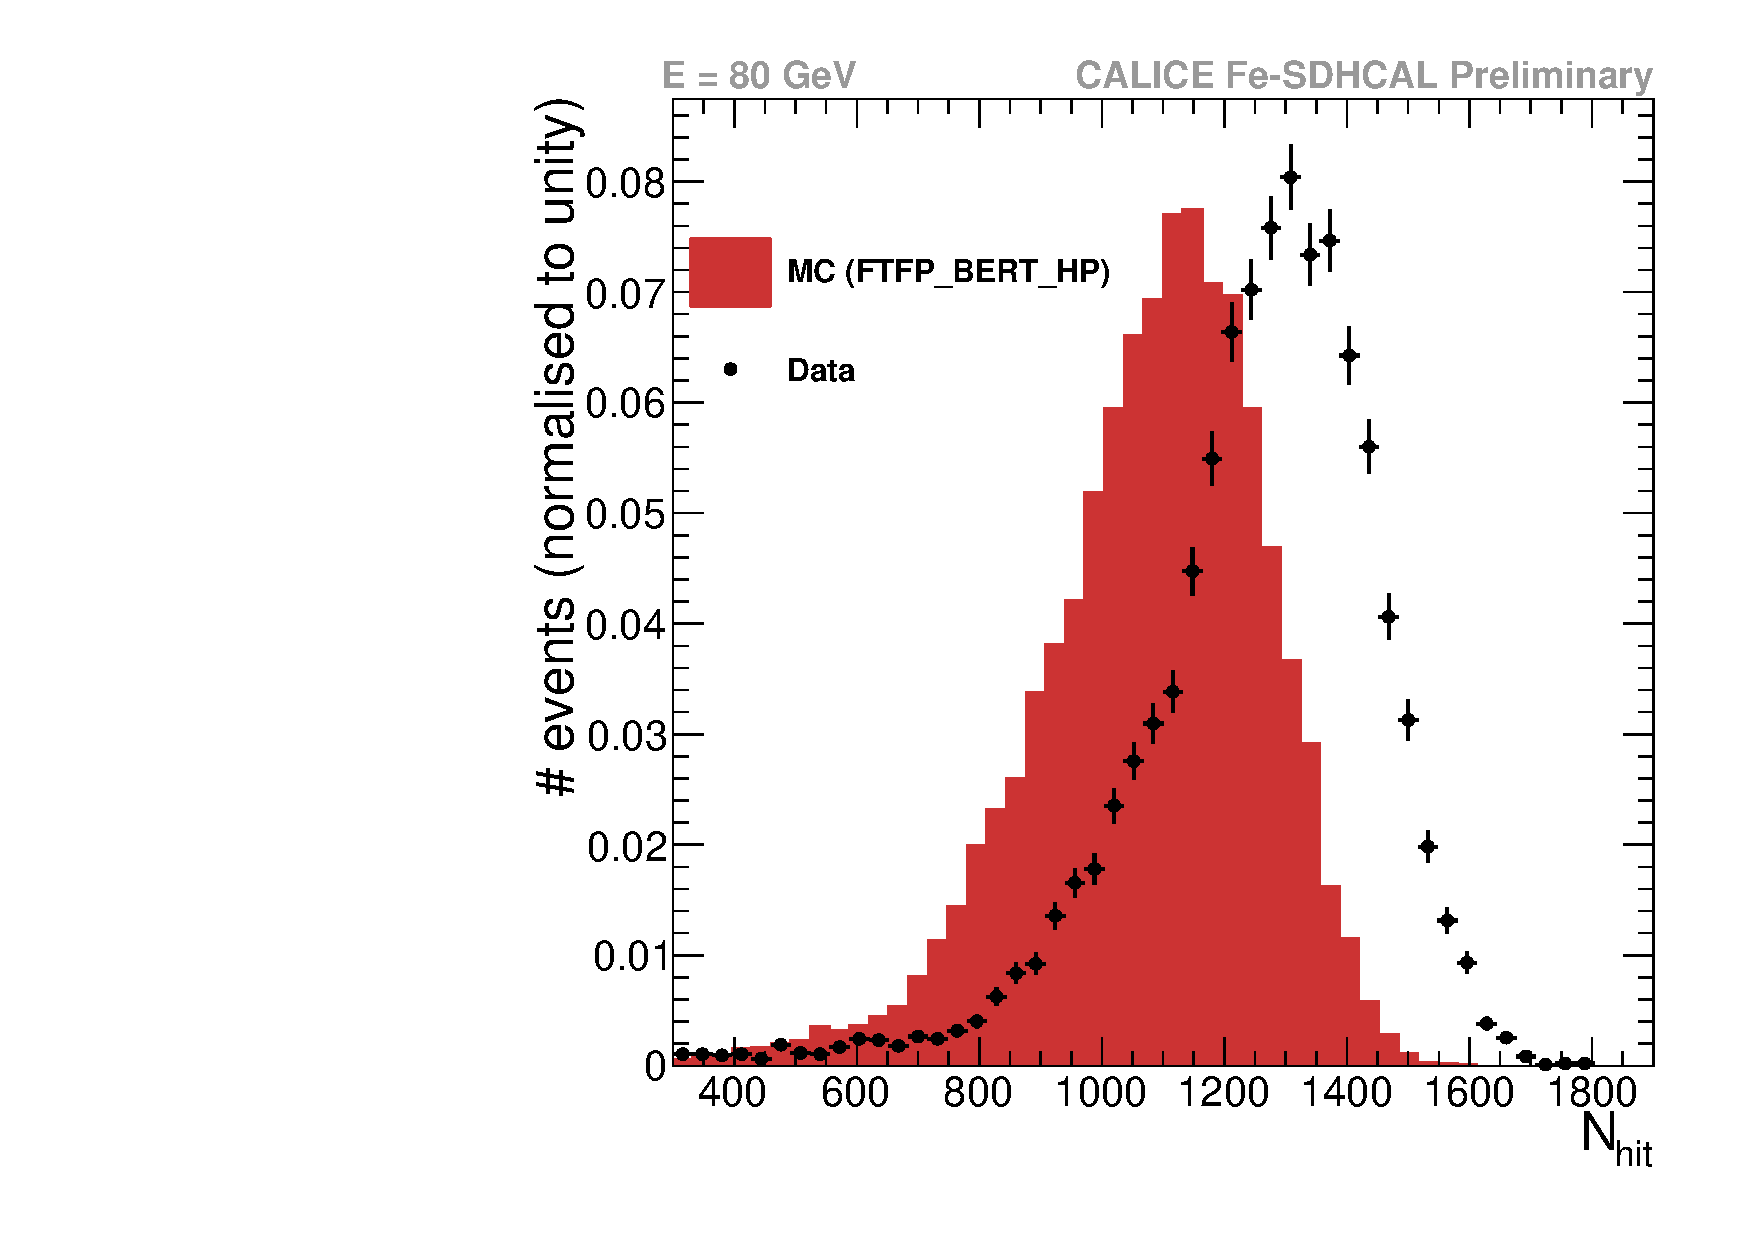
\includegraphics[width=.5\textwidth]{Digitizer/figs/nhit_pi-_80GeV_AugSep2012.pdf}}
  \caption{Distribution du nombre de hits pour des échantillons de pions de 20 GeV (a), de 40 GeV(b), de 60 GeV (c) et de 80 GeV (d). Les données sont représentées par des croix noires et la simulation par les histogrammes rouges.\label{fig.pi-nhit}}
\end{figure}

\begin{figure}[!ht]
  \subfigure[]{\includegraphics[width=.5\textwidth]{Digitizer/figs/NHITPIONHP.pdf}}
  \subfigure[]{\includegraphics[width=.5\textwidth]{Digitizer/figs/NHITPROTON.pdf}}
  \caption{Moyenne du nombre de hits for des échantillons de pions en fonction de l'énergie du faisceau. Les données sont représentés par des croix noires et la simulation par des cercles rouges (FTFP\_BERT\_HP) et des carrés bleus (QGSP\_BERT\_HP). La déviation relative est aussi présentée. (a) : données enregistrées sur la ligne H6 du SPS au CERN; (b) : données enregistrées sur la ligne H2 du SPS au CERN.}
  \label{fig.nhit_pi-_ebeam}
\end{figure}

%%%%%%%%%%%%%%%%%%%%%%%%%%%%%%%%%%%%%%%%%%%%%%%

\section{Conclusion}
